
\documentclass[xcolor=dvipsnames,10pt,compress,aspectratio=169]{beamer}
\usepackage[utf8]{inputenc}
%\usepackage[brazilian]{babel}
\usepackage{verbatim}
\usepackage{graphicx}
\usepackage{xspace}
\usepackage{color}
\usepackage{amsthm}
\usepackage{url}
\usepackage{array}
\usepackage{hyperref}
\usepackage{times,mathptmx}
\usepackage{multimedia}
\usepackage{framed}
%\usetheme{Madrid}
%\usetheme{Boadilla}
\usetheme{Darmstadt}
%\usetheme{Frankfurt}
%\usetheme{CambridgeUS}
%\usetheme{AnnArbor}
%\usecolortheme{beaver}
%\usecolortheme{seahorse}
%\usecolortheme{seagull}

\setbeamercovered{transparent}
\setbeamertemplate{footline}[frame number]
\setbeamertemplate{navigation symbols}{}
\usecolortheme[named=BrickRed]{structure}

%\setbeamertemplate{footline}[frame number]
%\setbeamersize{text margin left=1em,text margin right=1em}

\newcommand{\disciplina}{Prática em Sistemas Operacionais}
\newcommand{\aula}{Introdução - Redes de Computadores}
\newcommand{\nome}{João Vicente Ferreira Lima}

\lecture[1]{\aula}{aula02}
\def\lecturename{\aula}

\newcommand{\Red}[1]{{\color{red}#1}}
\newcommand{\red}[1]{{\color{red}#1}}
\newcommand{\Blue}[1]{{\color{blue}#1}}
\newcommand{\blue}[1]{{\color{blue}#1}}

\newcommand{\PBS}[1]{\let\temp=\\#1\let\\=\temp}
\newcommand{\RRCOL}{\PBS\raggedright\hspace{0pt}}

\title[\aula]{\aula}

\subtitle{\disciplina}

\author[João Vicente Ferreira Lima]{\nome}

\institute[UFSM]{Departamento de Linguagens e Sistemas de Computação \\ Universidade Federal de Santa Maria \\ \url{jvlima@inf.ufsm.br}}
\date{2021/2}

\graphicspath{{.}{figs/}{../logos/}}

\logo{
    
\includegraphics[height=1cm,width=1cm,keepaspectratio]{logo_inf}
    
\includegraphics[height=1cm,width=1cm,keepaspectratio]{logo_ufsm}
}

\newtheorem{mydef}{Definição}[section]
%\newtheorem{myteo}{Teorema}[section]

% Typesetting Listings
\usepackage{listings}
\lstset{%
language=Python,
basicstyle=\small\ttfamily,
commentstyle=\slshape\color{green!50!black},
keywordstyle=\bfseries\color{blue!50!black},
stringstyle=\color{red},
numbers=left,
% escapechar=\#,
breaklines=false,
emphstyle=\color{red}
}

\begin{document}

\begin{frame}
  \maketitle
\end{frame}

%%%%%%%%%%%%%%%%%%%%%%%%%%%%%%%%%%%%%%%%%%%%%%%%%%%%%%%%%%%%%%%%%%%%%%%%%%%%%%%

\frame{
    \frametitle<presentation>{Sumário}
    \tableofcontents[hideallsubsections]
}

\AtBeginSection{
  \begin{frame}
    \frametitle{Sumário}
    \tableofcontents[currentsection,hideothersubsections]
  \end{frame}
}

\AtBeginSubsection{
  \begin{frame}
    \frametitle{Sumário}
    \tableofcontents[currentsection,currentsubsection]
  \end{frame}
}

%%%%%%%%%%%%%%%%%%%%%%%%%%%%%%%%%%%%%%%%%%%%%%%%%%%%%%%%%%%%%%%%%%%%%%%%%%%%%%%
\section{Fundamentos em Redes}
%%%%%%%%%%%%%%%%%%%%%%%%%%%%%%%%%%%%%%%%%%%%%%%%%%%%%%%%%%%%%%%%%%%%%%%%%%%%%%%

%-----------------------------------------------------------------------------%
\subsection{Introdução}
%-----------------------------------------------------------------------------%

\begin{frame}
  \frametitle{Problemas de redes para sistemas distribuídos}
  \begin{itemize}
  \item {\bf Desempenho} - latência, taxa de transferência.
  \item {\bf Escalabilidade} - tamanho, geográfica e administrativa.
  \item {\bf Confiabilidade} - erros em hardware e software.
  \item {\bf Segurança} - firewall, criptografia, VPNs (\emph{virtual private network}).
  \item {\bf Mobilidade} -  dispositivos móveis e laptops.
  \item {\bf Qualidade de Serviço (QoS)} - largura de banda e latência.
  \item {\bf Multicasting} (\emph{difusão seletiva}) - comunicação um-para-muitos.
  \end{itemize}
\end{frame}

%---------------------------------------------------------------------
\begin{frame}
  \frametitle{Tipos de redes}
  \begin{figure}[ht]
\alt<presentation>
{
  \begin{center}
  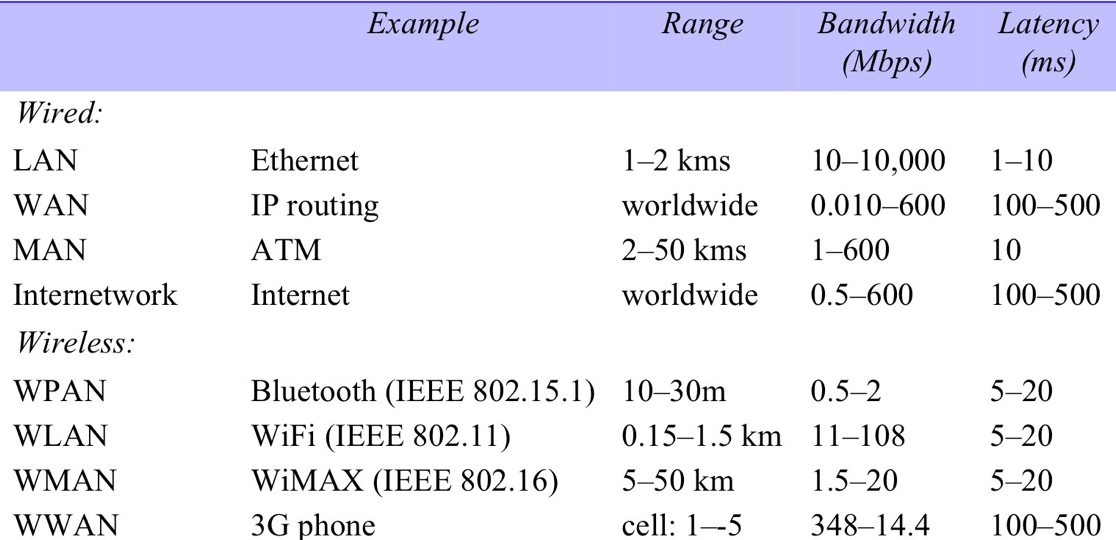
\includegraphics[width=0.8\textwidth]{chap3-01-coulouris}
  \end{center}
}
{
  \begin{center}
  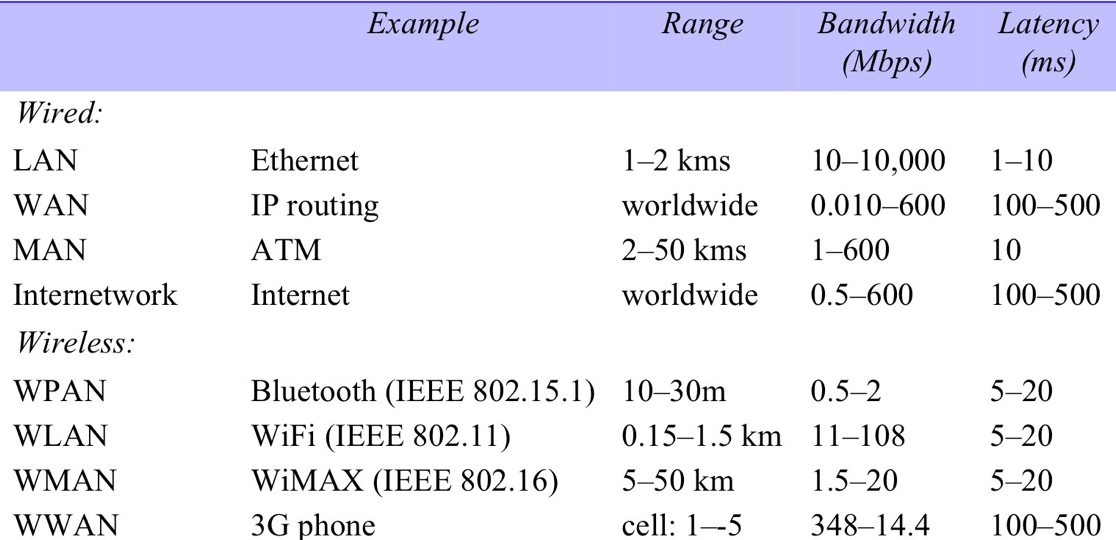
\includegraphics[width=0.6\textwidth]{chap3-01-coulouris}
  \end{center}
}
  \end{figure}
\end{frame}

%-----------------------------------------------------------------------------%
\subsection{Protocolos em camadas}
%-----------------------------------------------------------------------------%

\begin{frame}
  \frametitle{Fundamentos}
  \begin{itemize}
  \item Toda comunicação em sistemas distribuídos é baseada em mensagens (de baixo nível)
  \item Para que a comunicação seja bem sucedida deve haver \textbf{regras}
    \begin{itemize}
    \item Essas regras são \textbf{protocolos}
    \item Diversos aspectos a considerar (tamanho da mensagem, erros, pacotes, etc)
    \end{itemize}
% TODO
% orientado a conexao, ou nao
  \end{itemize}
  %
\end{frame}

\begin{frame}
  \frametitle{Modelo de referência básico}
\only<presentation>
{
  \vspace{-2mm}
}
  \begin{figure}[ht]
  \centering
  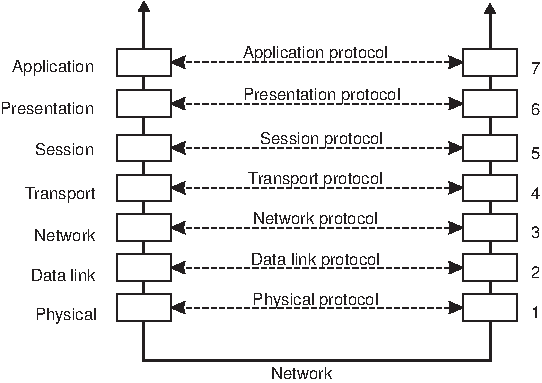
\includegraphics[scale=0.8]{04-01}
  \end{figure}
\only<presentation>
{
  \vspace{-2mm}
}
  \pause
  %
  \begin{block}{Modelo OSI}
    \begin{itemize}
    \item {\bf Modelo de referência para interconexão de sistemas abertos} ou \textbf{ISO OSI}
    \item Nunca foram amplamente utilizados
    \end{itemize}
  \end{block}
\end{frame}

\begin{frame}
  \frametitle{Pilha de protocolos}
  \begin{figure}[ht]
  \centering
  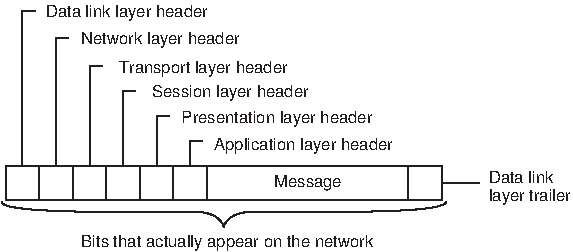
\includegraphics[scale=0.9]{04-02}
  \end{figure}
  \pause
  \begin{block}{Protocolos em camadas}
    \begin{itemize}
    \item Protocolos de níveis mais baixos
    \item Protocolos de transporte
    \item Protocolos de níveis mais altos
    \item Protocolos de middleware
    \end{itemize}
  \end{block}
\end{frame}

\begin{frame}
  \frametitle{Protocolos de níveis mais baixos}
  \begin{itemize}
  \item \blue{Camada física} - especificação e implementação de bits, além da transmissão. Ex: Ethernet, Wi-Fi, etc.
  \item \blue{Camada de enlace} - efetua a transmissão de uma série de
    bits agrupados em \textbf{quadros} (\emph{frame}), bem como sequencia e verificação de erros. Ex: MAC, ARP, etc.
  \item \blue{Camada de rede} - descreve como pacotes em uma rede de computadores são 
    \textbf{roteados}. Ex: ICMP, IP, etc.
  \end{itemize}
  %
  \pause
  \begin{alertblock}{Observação}
  Para muitos sistemas distribuídos, a camada mais baixa é a camada de rede.
  \end{alertblock}
  \begin{exampleblock}{Observação}
  O protocolo de rede mais utilizado atualmente é o {\bf protocolo de Internet (Internet Protocol - IP)}, sem conexão
  que faz parte da pilha de protocolos da Internet. Um \textbf{pacote} IP pode sem enviado sem preparação alguma.
  \end{exampleblock}
\end{frame}


%-----------------------------------------------------------------------------%
\subsection{Camada de rede}
%-----------------------------------------------------------------------------%

\begin{frame}
  \frametitle{Camada de rede}
\alt<presentation>
{
  \centering
  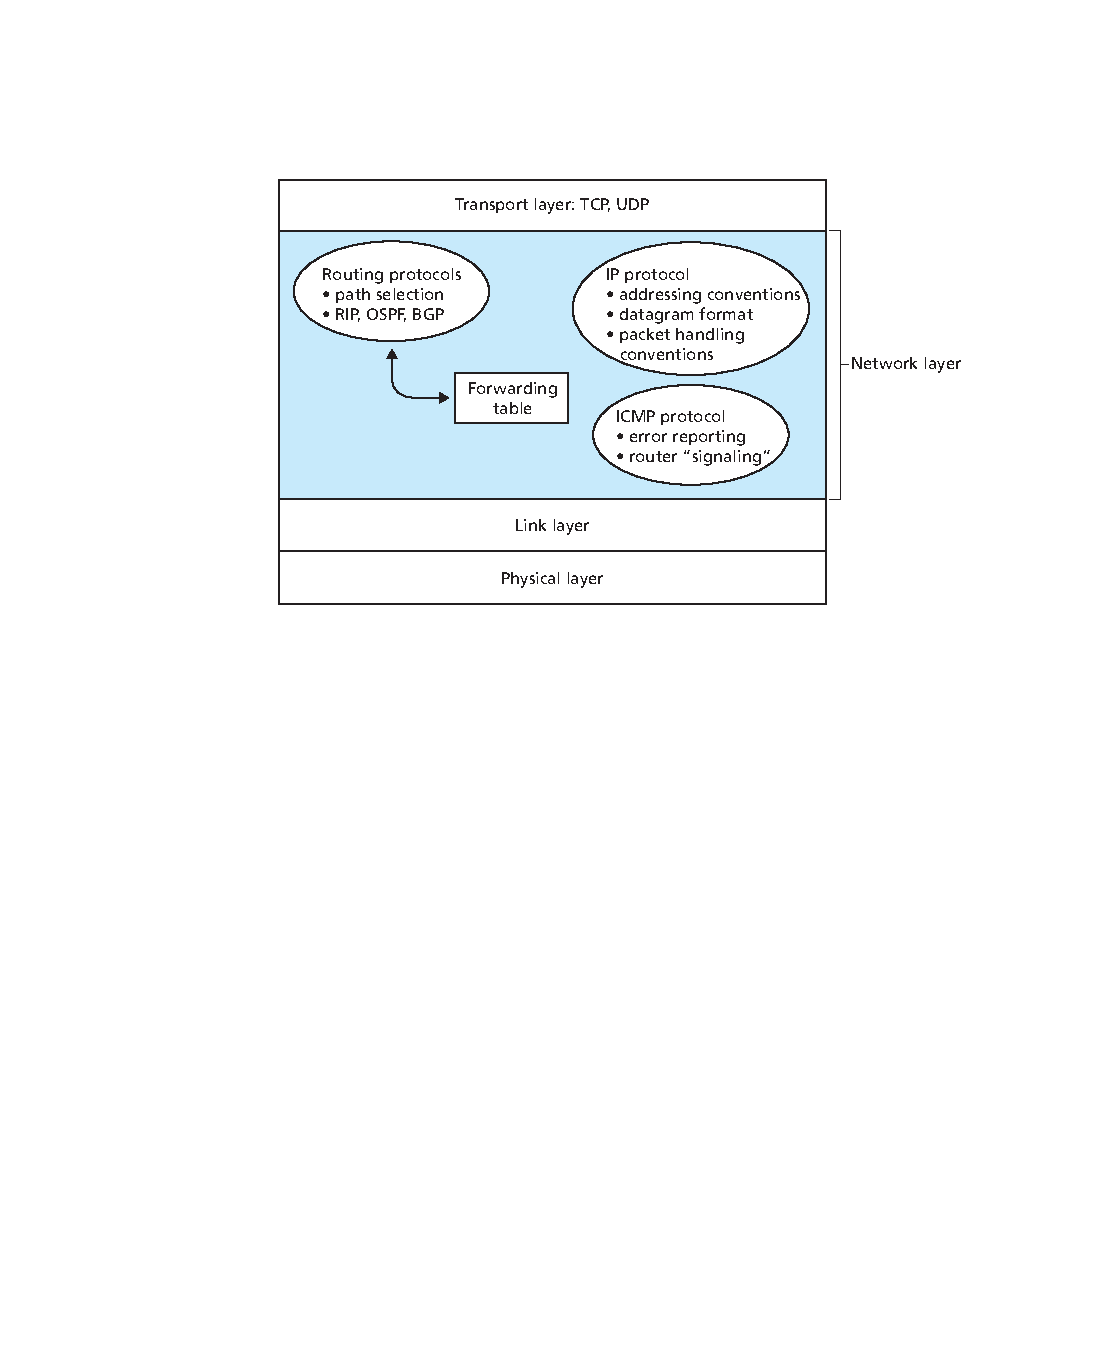
\includegraphics[width=0.8\textwidth]{kurose-04-01}
}
{
  \begin{figure}[ht]
  \centering
  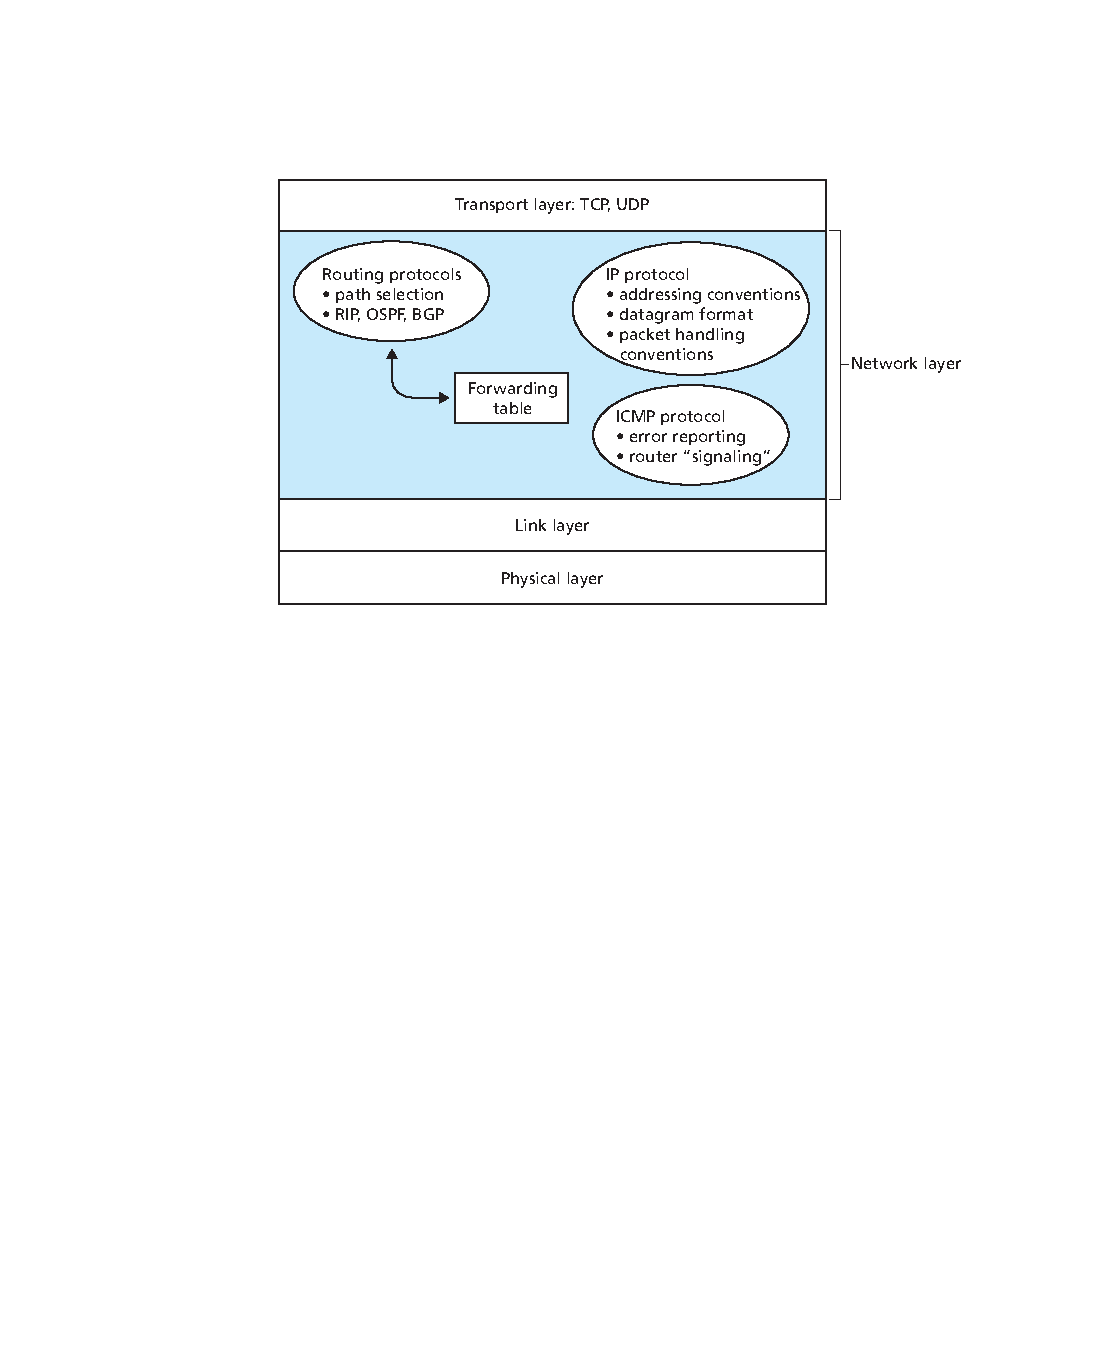
\includegraphics[width=0.6\textwidth]{kurose-04-01}
  \end{figure}
}
\end{frame}

\begin{frame}
  \frametitle{IP version 4 (IPv4)}
\alt<presentation>
{
  \centering
  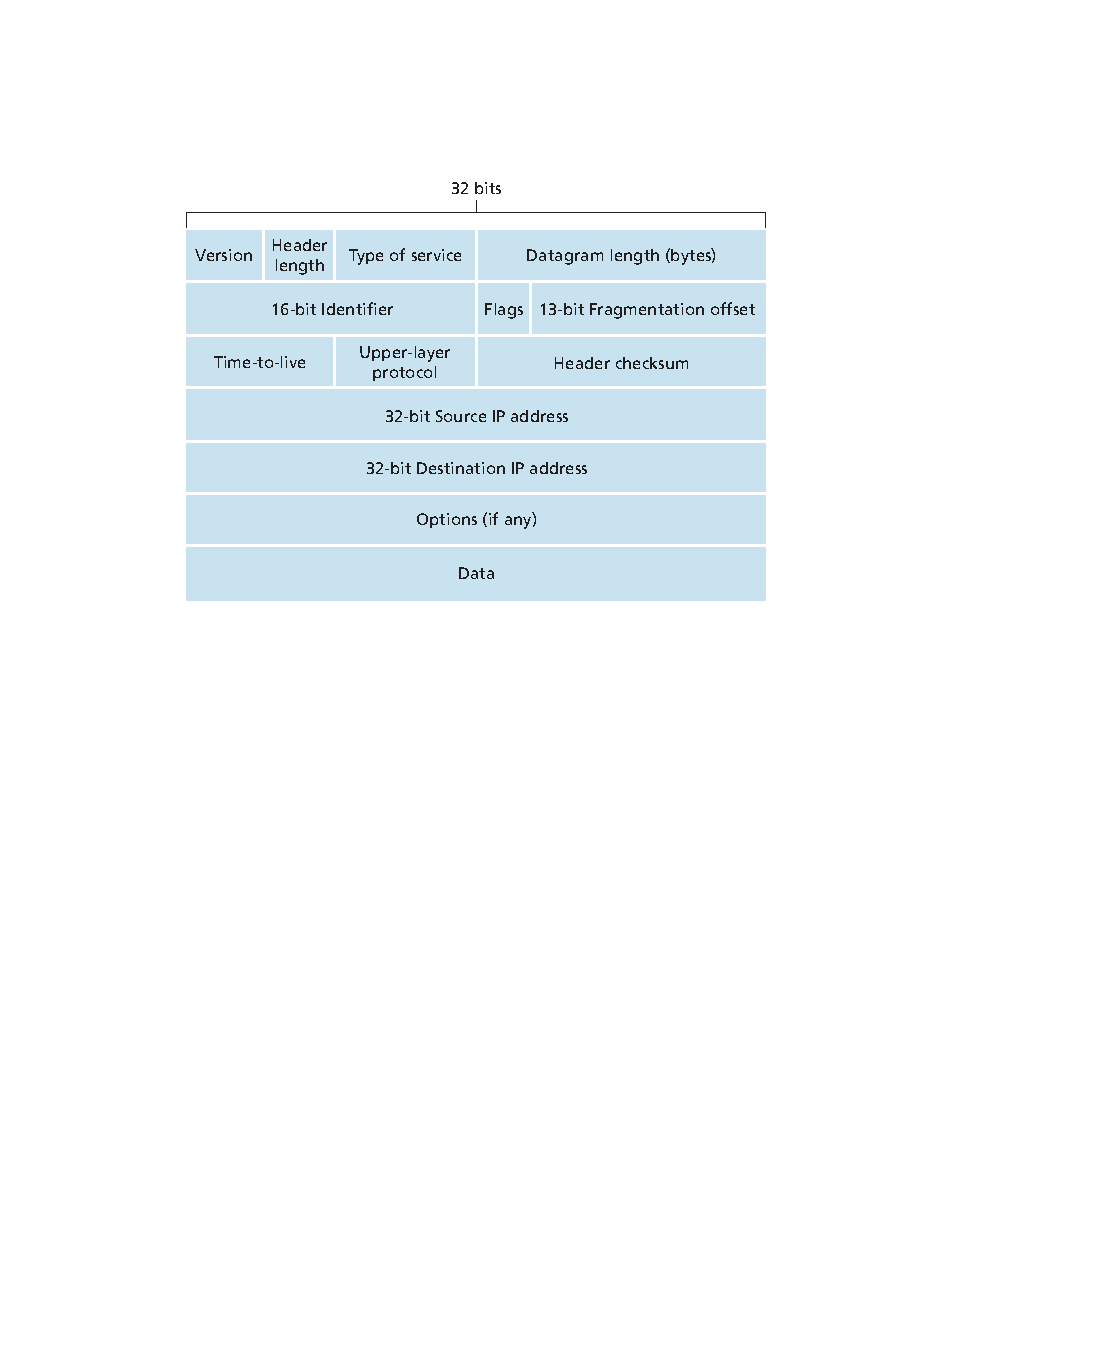
\includegraphics[width=0.6\textwidth]{kurose-04-02}
}
{
  \begin{figure}[ht]
  \centering
  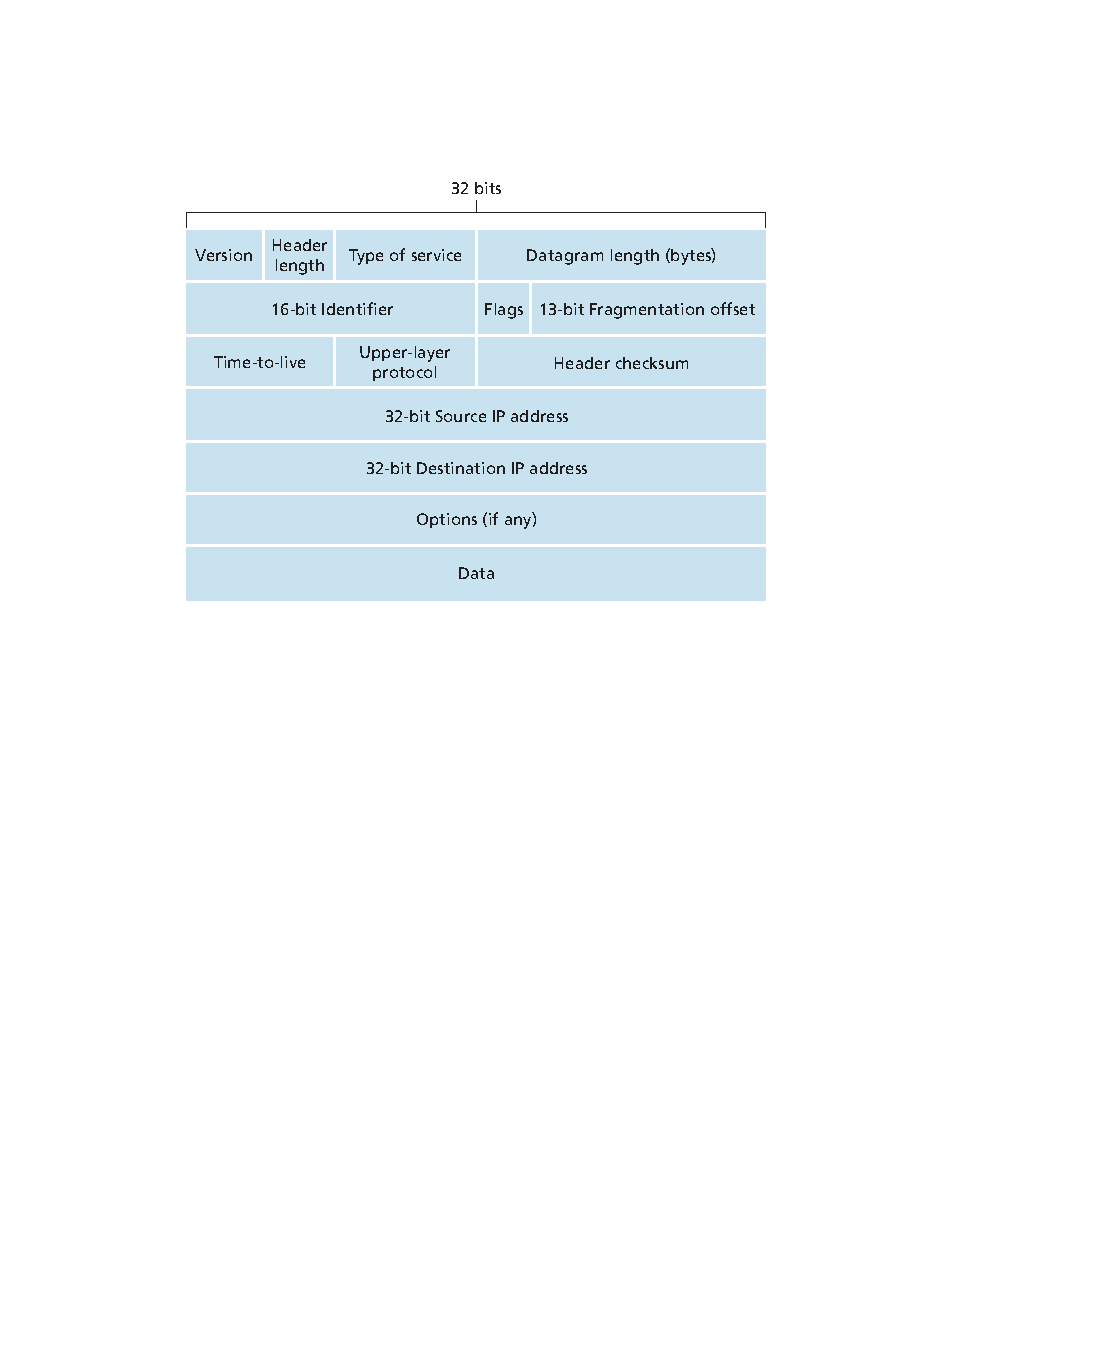
\includegraphics[width=0.6\textwidth]{kurose-04-02}
  \end{figure}
}
\end{frame}

\begin{frame}
  \frametitle{IP version 4 (IPv4)}
  \begin{itemize}
  \item Cabeçalho IP tem 20 bytes e TCP 20 bytes = 40 bytes + outras camadas.
  \item \textbf{IP Datagram Fragmentation} - os pacotes IP são fragmentados para transmissão
  \item O máximo de dados em um quadro da camada de enlace é o \emph{maximum transmission unit} (\textbf{MTU})
    \begin{itemize}
    \item O tamanho do frame Ethernet é de \textbf{1500 bytes}
    \end{itemize}
  \end{itemize}
\end{frame}

\begin{frame}[fragile]
  \frametitle{IP version 4 (IPv4)}
  \begin{itemize}
  \item Endereçamento de 32-bit = $2^{32}$ endereços IP.
  \item De \verb+0.0.0.0+ até \verb+255.255.255.255+.
  \end{itemize}
  \begin{block}{Endereçamento com 32-bit}
  \begin{center}
    \verb+11000001 00100000 11011000 00001001+\\
    equivalente ao IP \\
    \verb+193.32.21.216.9+
  \end{center}
  \end{block}
\end{frame}

\begin{frame}[fragile]
  \frametitle{IP Classless InterDomain Routing (CIDR)}
  \begin{itemize}
  \item CIDR generaliza a noção the subrede (subnet).
  \item Divide um enderaço 32-bit em duas partes com formato \verb+a.b.c.d/x+ onde \verb+x+
    indica o número de bits da primeira parte.
  \item A primeira parte é o prefixo (\textbf{prefix}).
  \end{itemize}
  \begin{exampleblock}{Exemplo de CIDR}
    \begin{itemize}
    \item \verb+10.1.1.0/24+ denota todos os endereços entre \verb+10.1.1.0+ e
      \verb+10.1.1.255+.
    \item O primeiro endereço (\verb+10.1.1.0+) é reservado para  identificar a rede (\emph{network address}).
    \item O último endereço (\verb+10.1.1.255+) é reservado para broadcast (\emph{broadcast address}).
    \item Os outros podem ser usados para computadores.
    \item Normalmente, o \verb+10.1.1.1+ é o router da rede.
    \end{itemize}
  \end{exampleblock}
\end{frame}

\begin{frame}[fragile]
  \frametitle{IP Classless InterDomain Routing (CIDR)}
  \begin{exampleblock}{Exemplo de CIDR}
    \begin{itemize}
    \item \verb+223.1.1.32/28+ denota todos os endereços entre \verb+223.1.1.32+ e
      \verb+223.1.1.47+.
    \item O primeiro endereço é reservado para  identificar a rede (\emph{network address}).
    \item O último endereço é reservado para broadcast (\emph{broadcast address}).
    \item Os  outros podem ser usados para computadores.
    \end{itemize}
  \end{exampleblock}
\end{frame}

\begin{frame}[fragile]
  \frametitle{IP Classless InterDomain Routing (CIDR)}
  \begin{itemize}
  \item {\bf Classe A} - redes muito grandes e longa distância em nível nacional. 
  \item {\bf Classe B} - organizações com mais que 255 computadores.
  \item {\bf Classe C} - usados nos demais tipos de redes.
  \item {\bf Classe D} - reservado para multicasting.
  \item {\bf Classe E} - reservado para uso futuro.
  \end{itemize}
\end{frame}

\begin{frame}
  \frametitle{IP Classless InterDomain Routing (CIDR)}
\alt<presentation>
{
  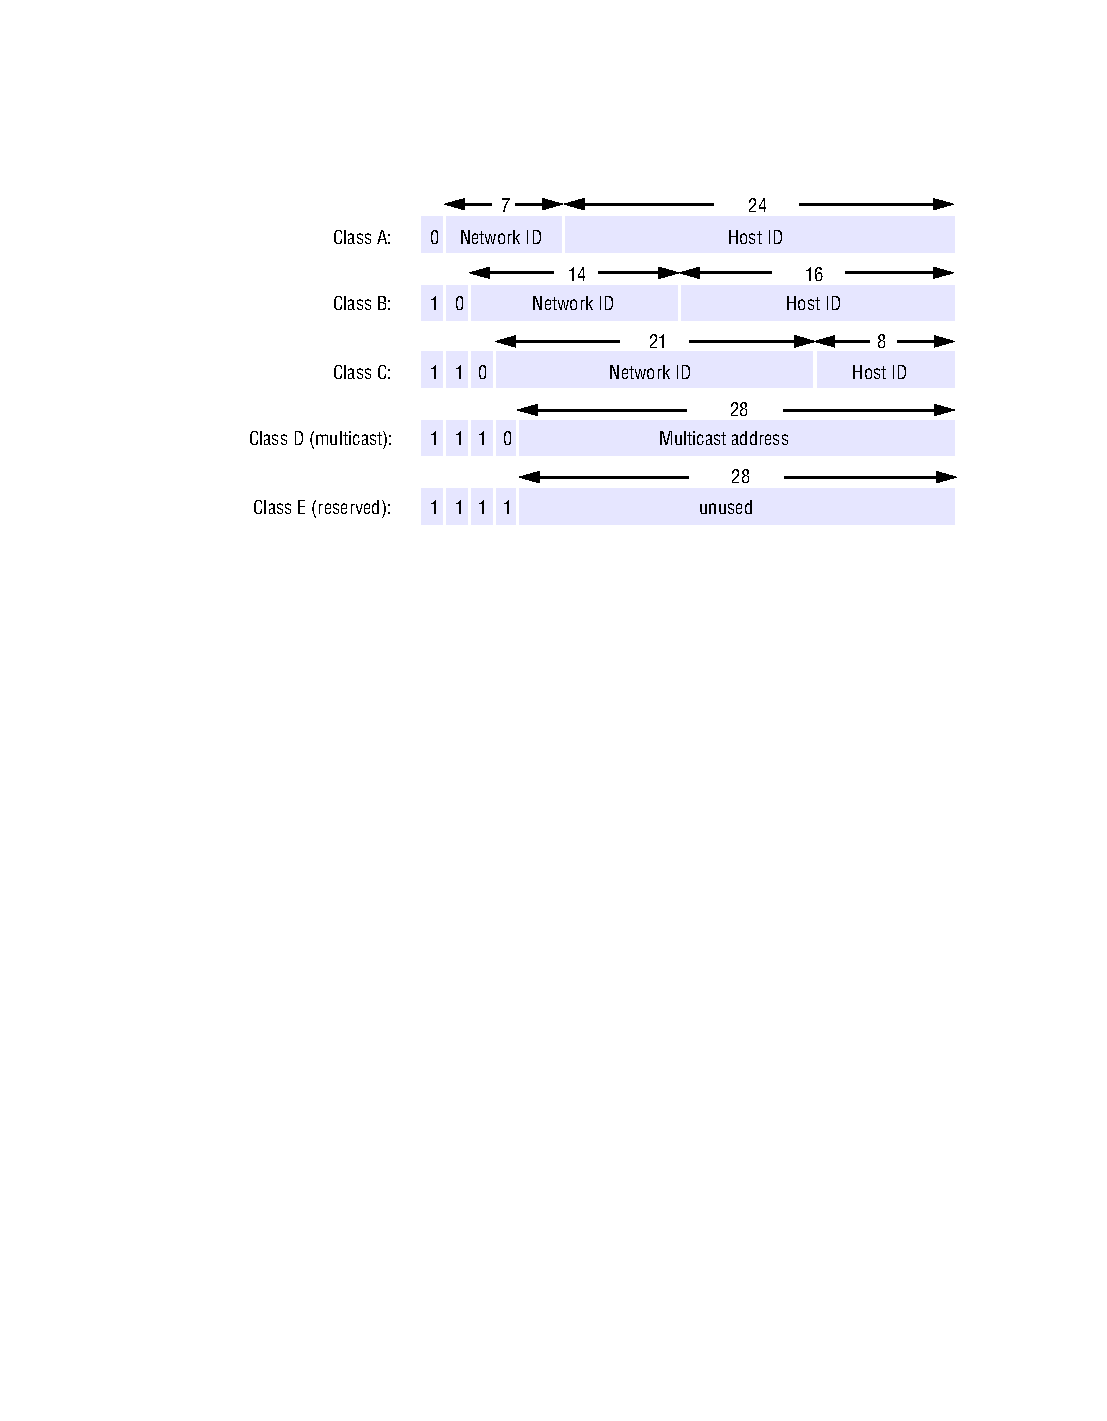
\includegraphics[width=\textwidth]{coulouris-03-15}
}
{
  \begin{figure}[ht]
  \centering
  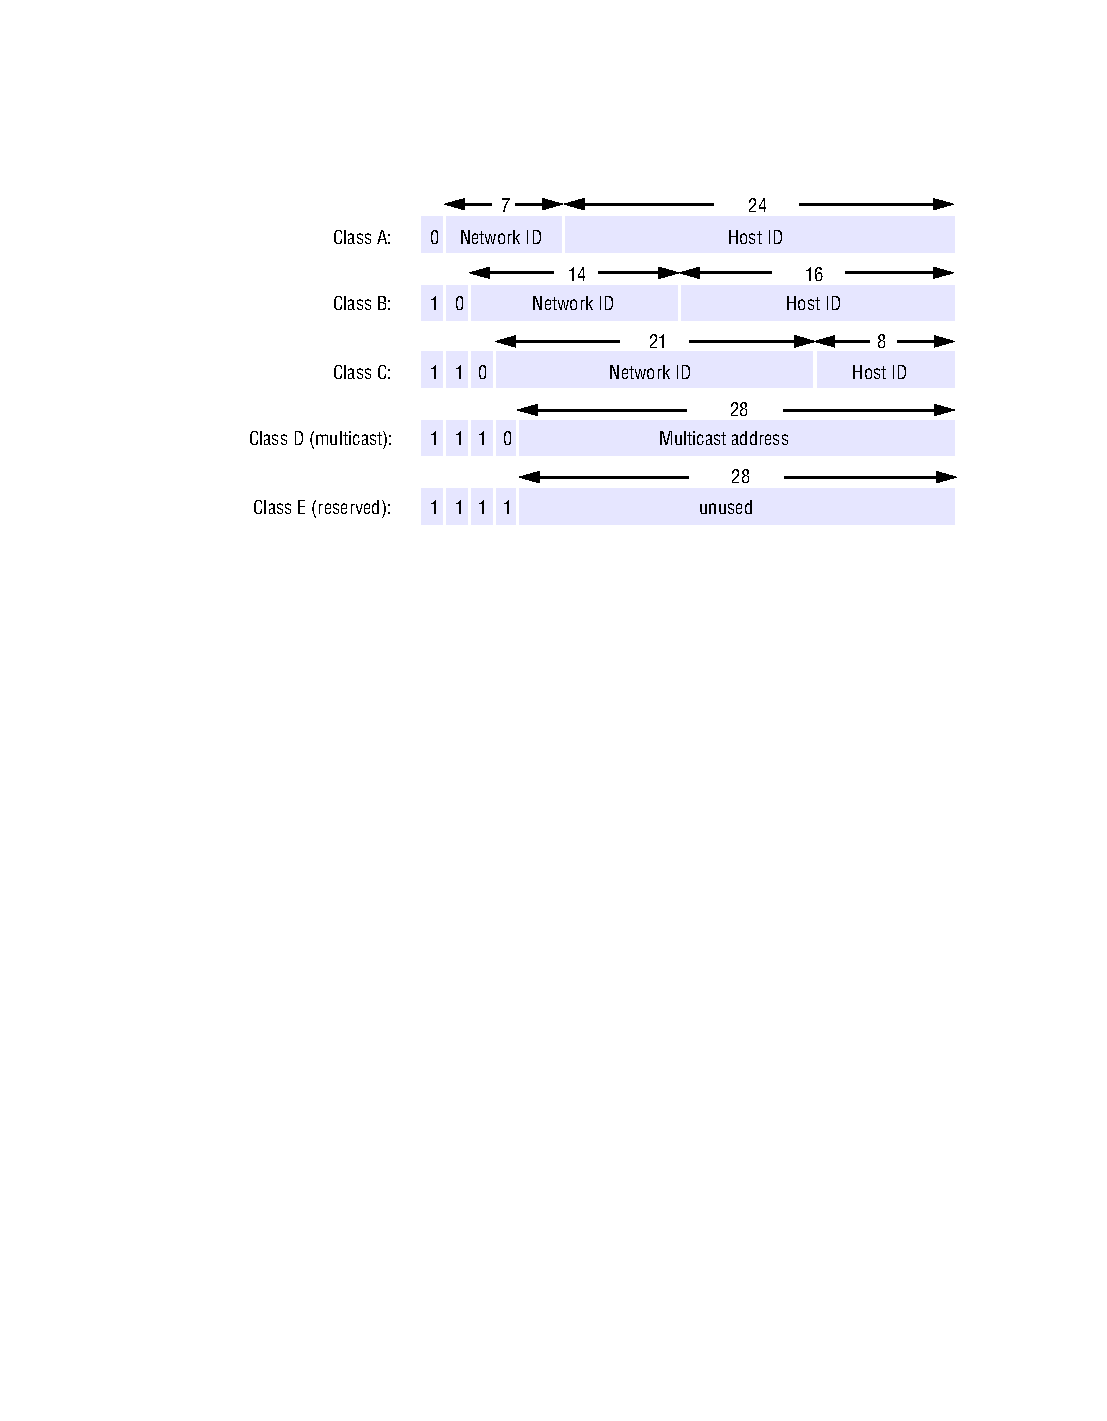
\includegraphics[width=0.6\textwidth]{coulouris-03-15}
  \end{figure}
}
\end{frame}

\begin{frame}
  \frametitle{IP Classless InterDomain Routing (CIDR)}
\alt<presentation>
{
  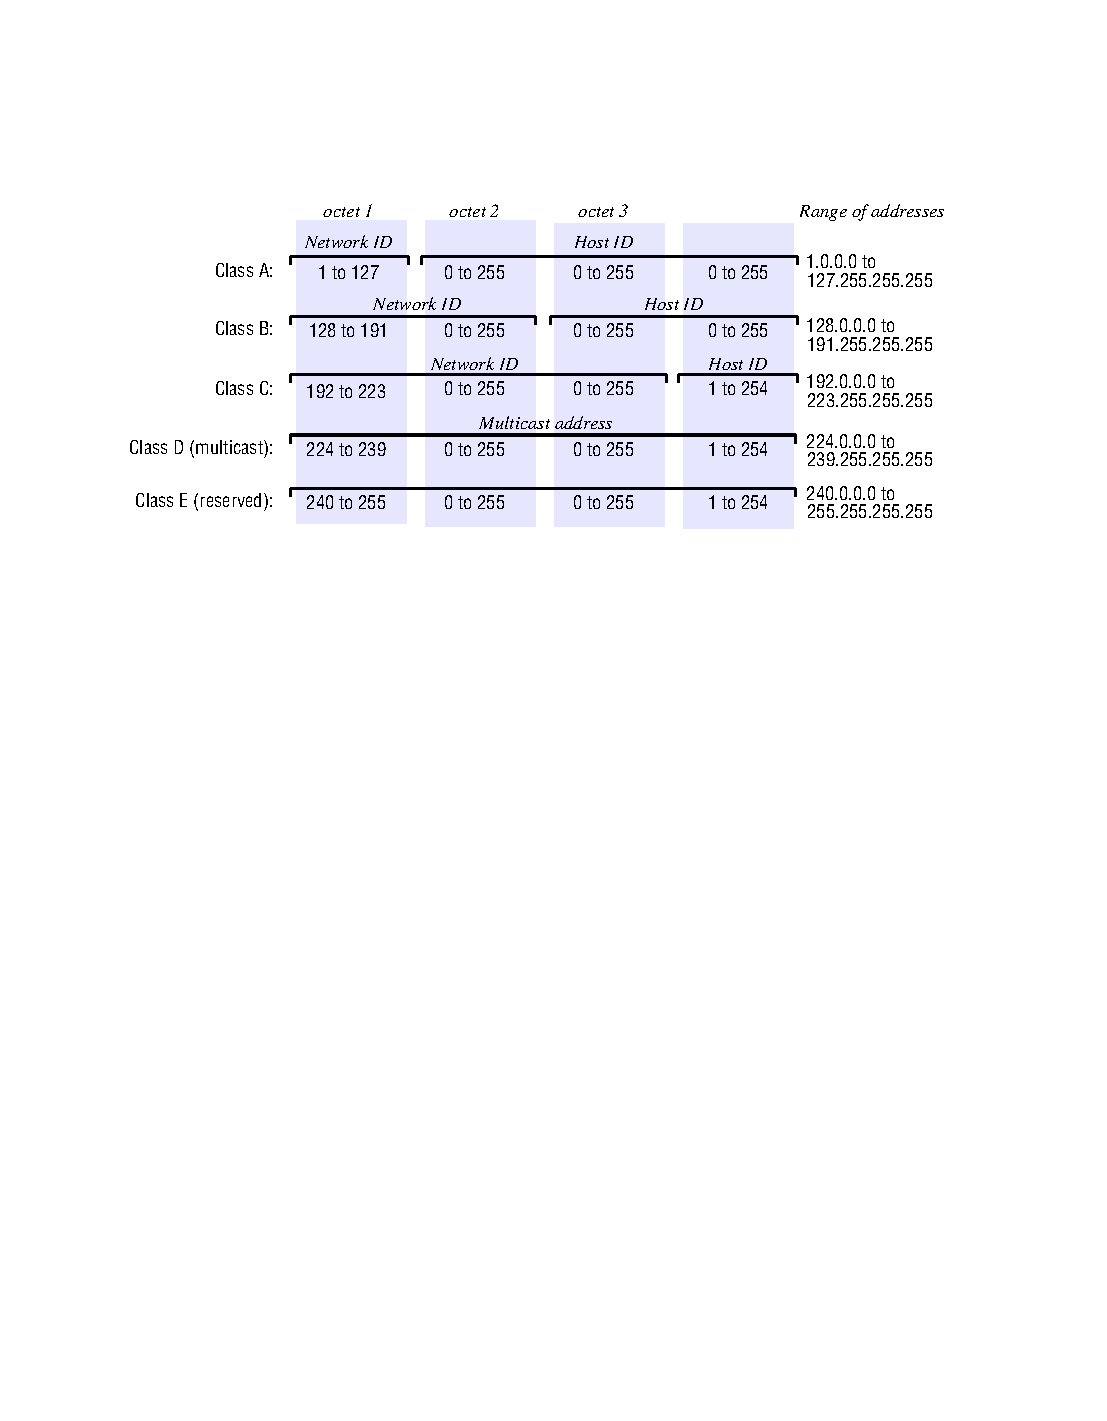
\includegraphics[width=\textwidth]{coulouris-03-16}
}
{
  \begin{figure}[ht]
  \centering
  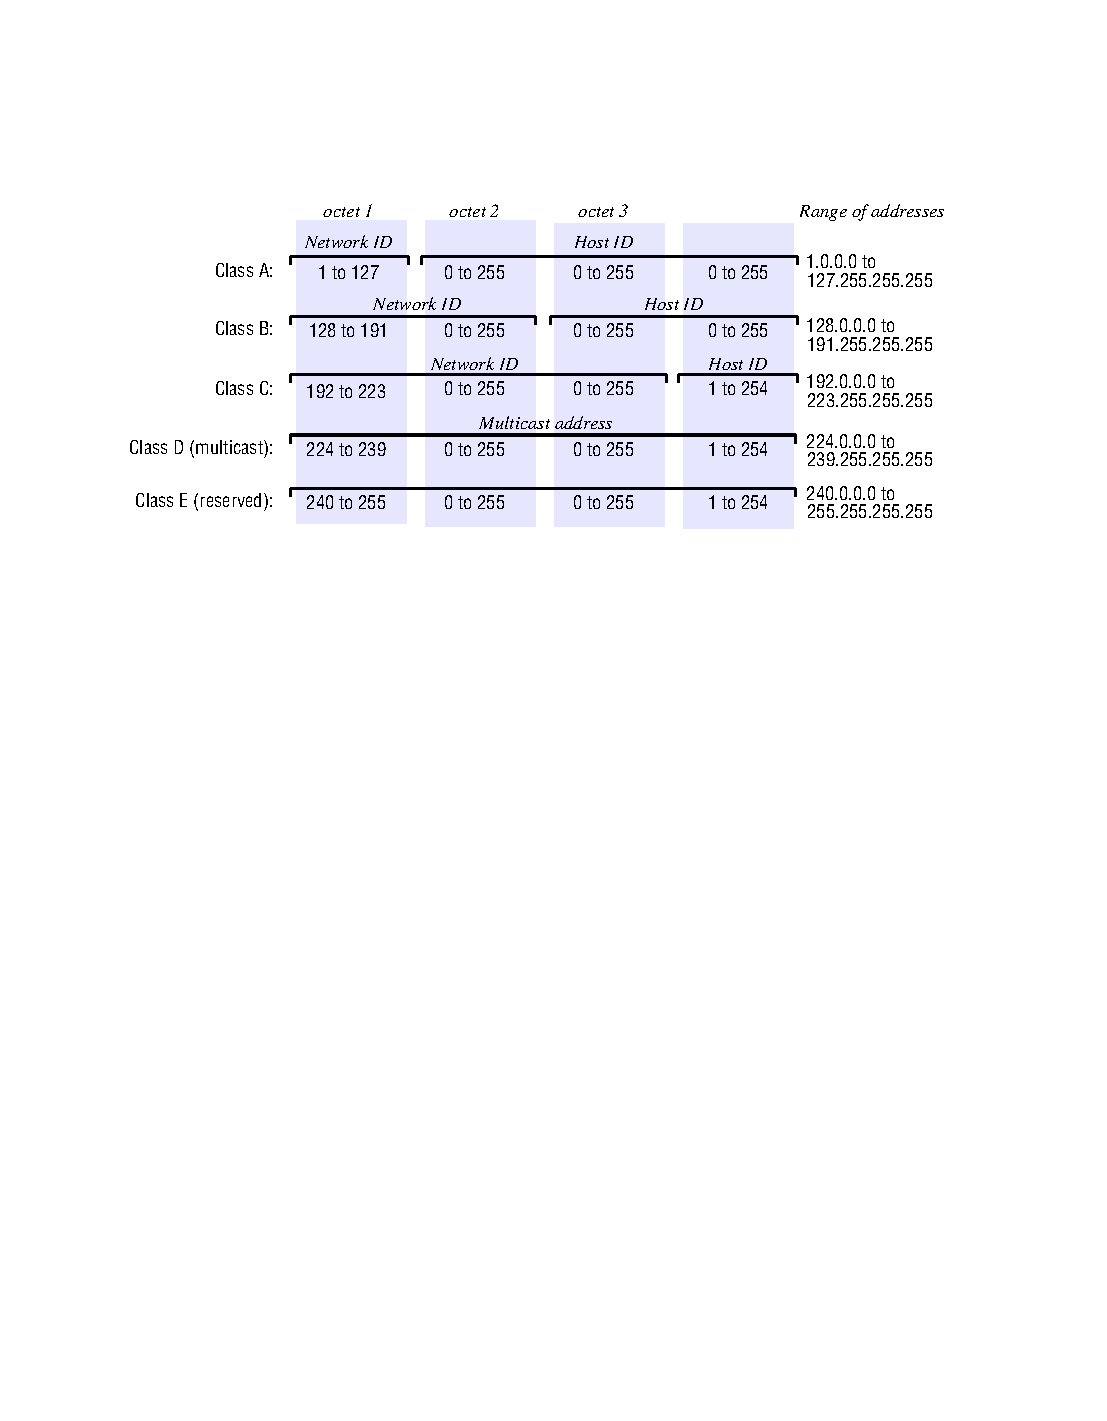
\includegraphics[width=0.6\textwidth]{coulouris-03-16}
  \end{figure}
}
\end{frame}

\begin{frame}
  \frametitle{Network Address Translation (NAT)}
\alt<presentation>
{
  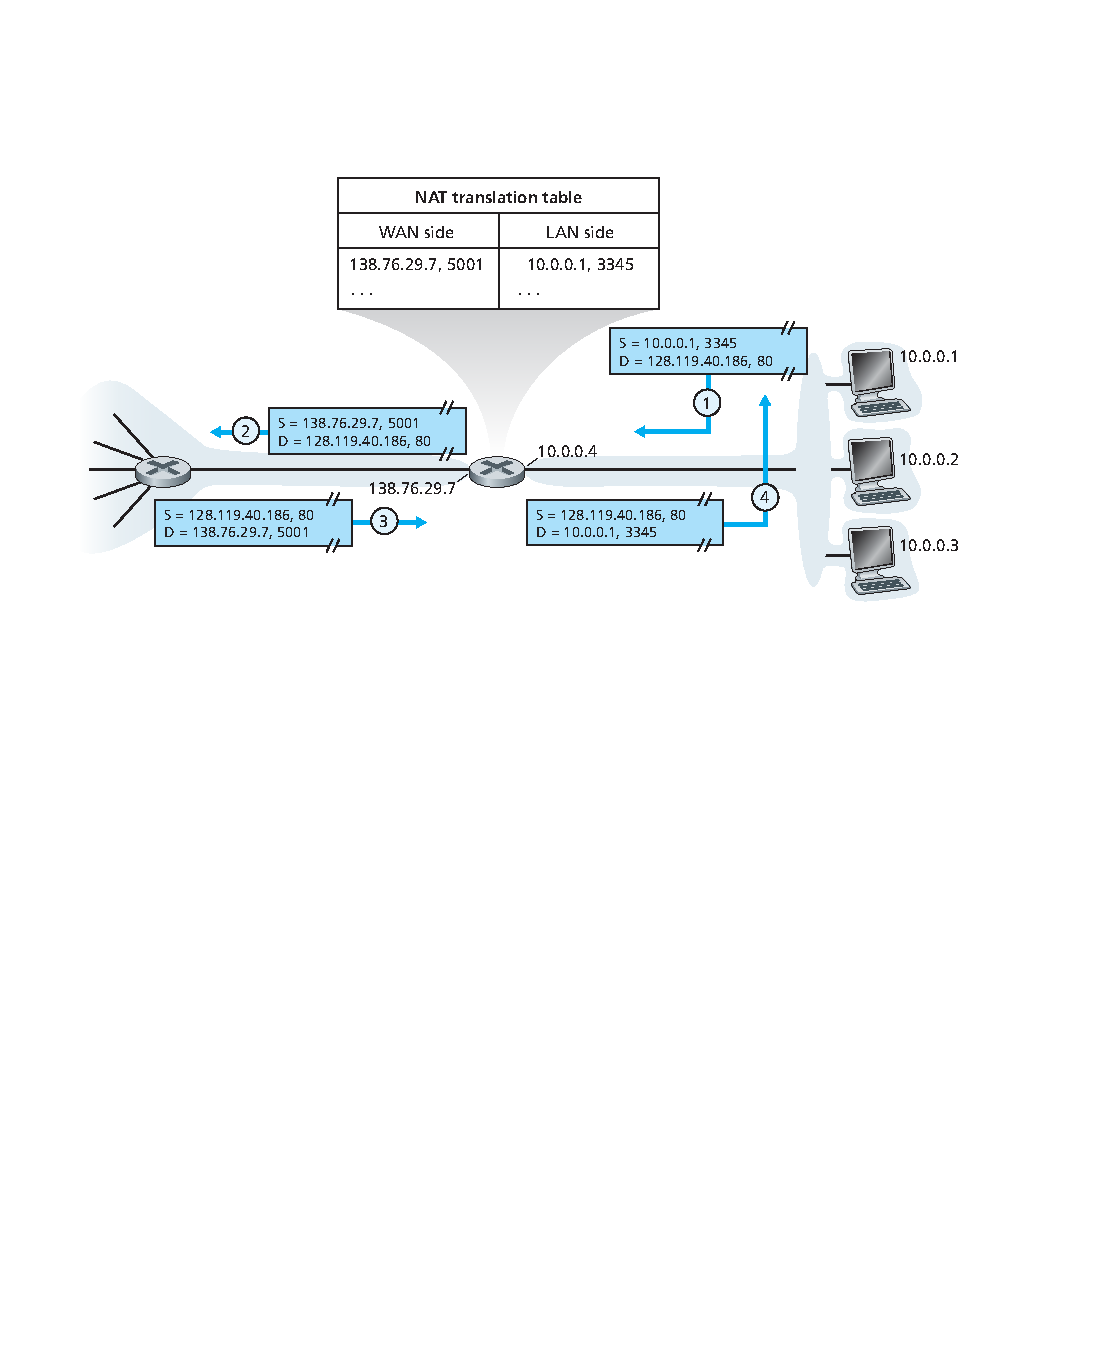
\includegraphics[width=\textwidth]{kurose-04-22}
}
{
  \begin{figure}[ht]
  \centering
  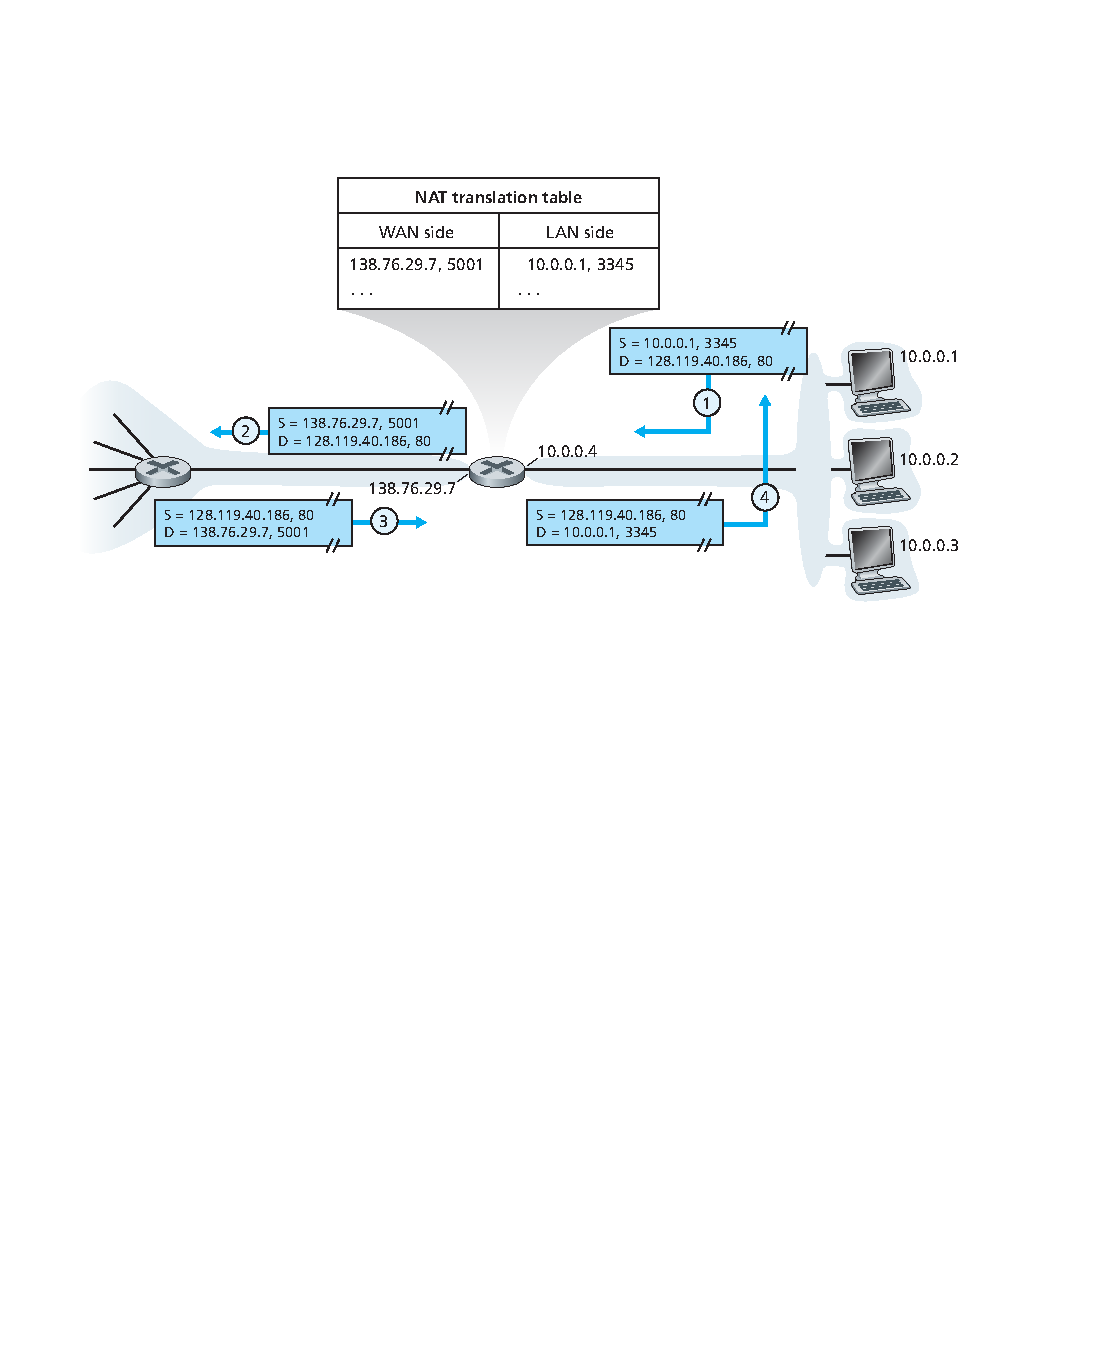
\includegraphics[width=0.6\textwidth]{kurose-04-22}
  \end{figure}
}
\end{frame}

\begin{frame}
  \frametitle{IP version 6 (IPv6)}
\alt<presentation>
{
  \centering
  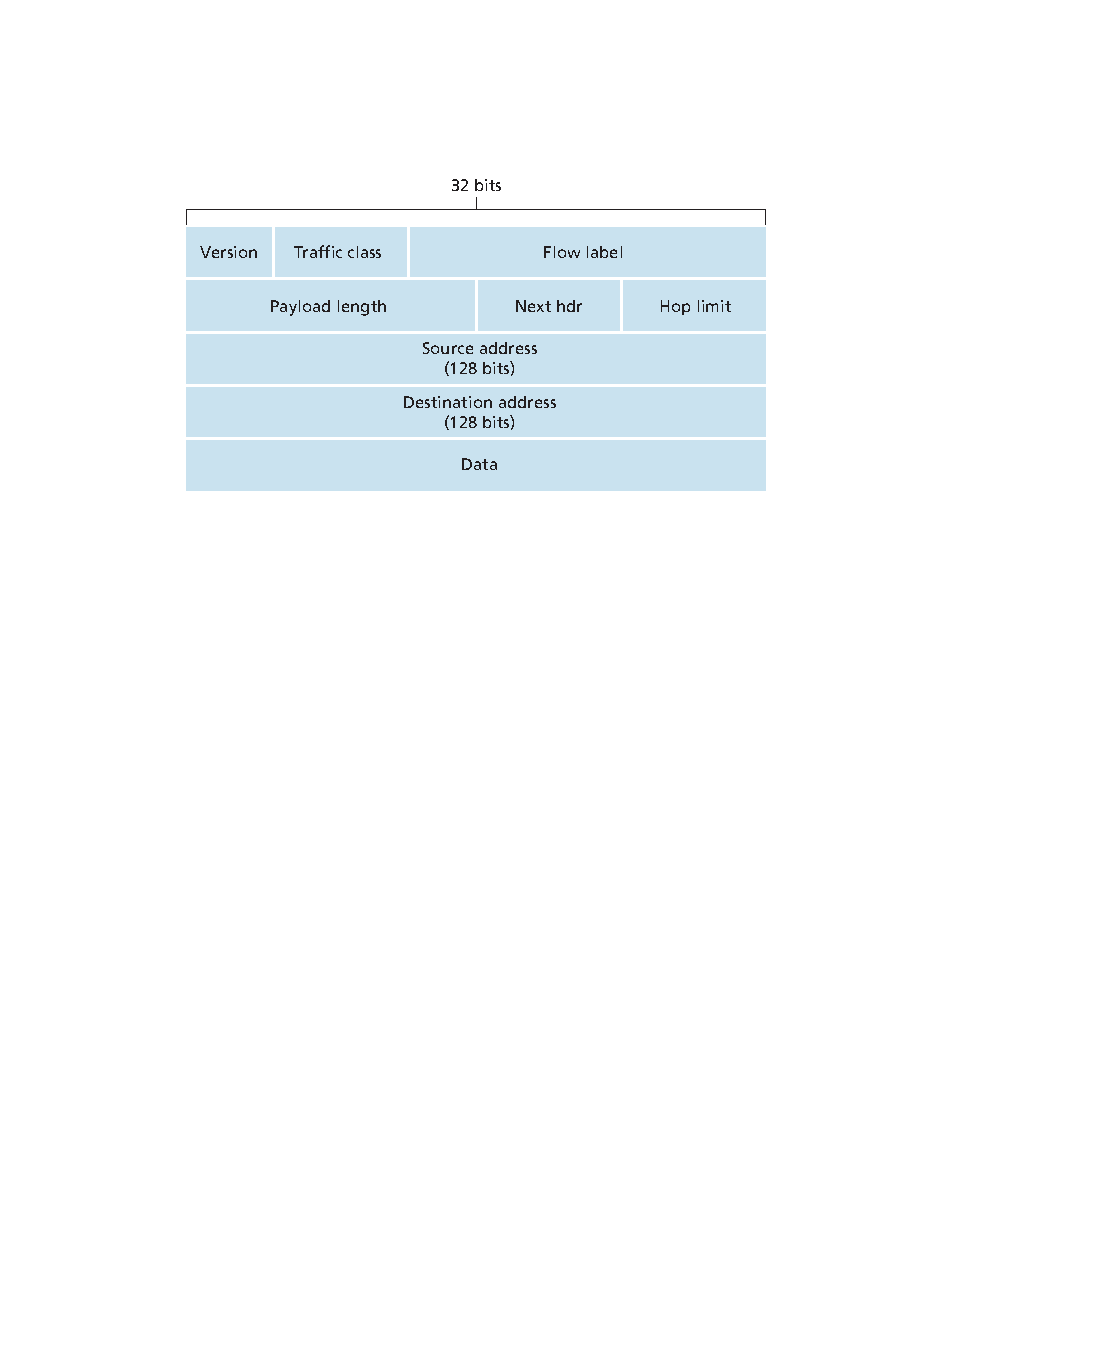
\includegraphics[width=0.8\textwidth]{kurose-04-24}
}
{
  \begin{figure}[ht]
  \centering
  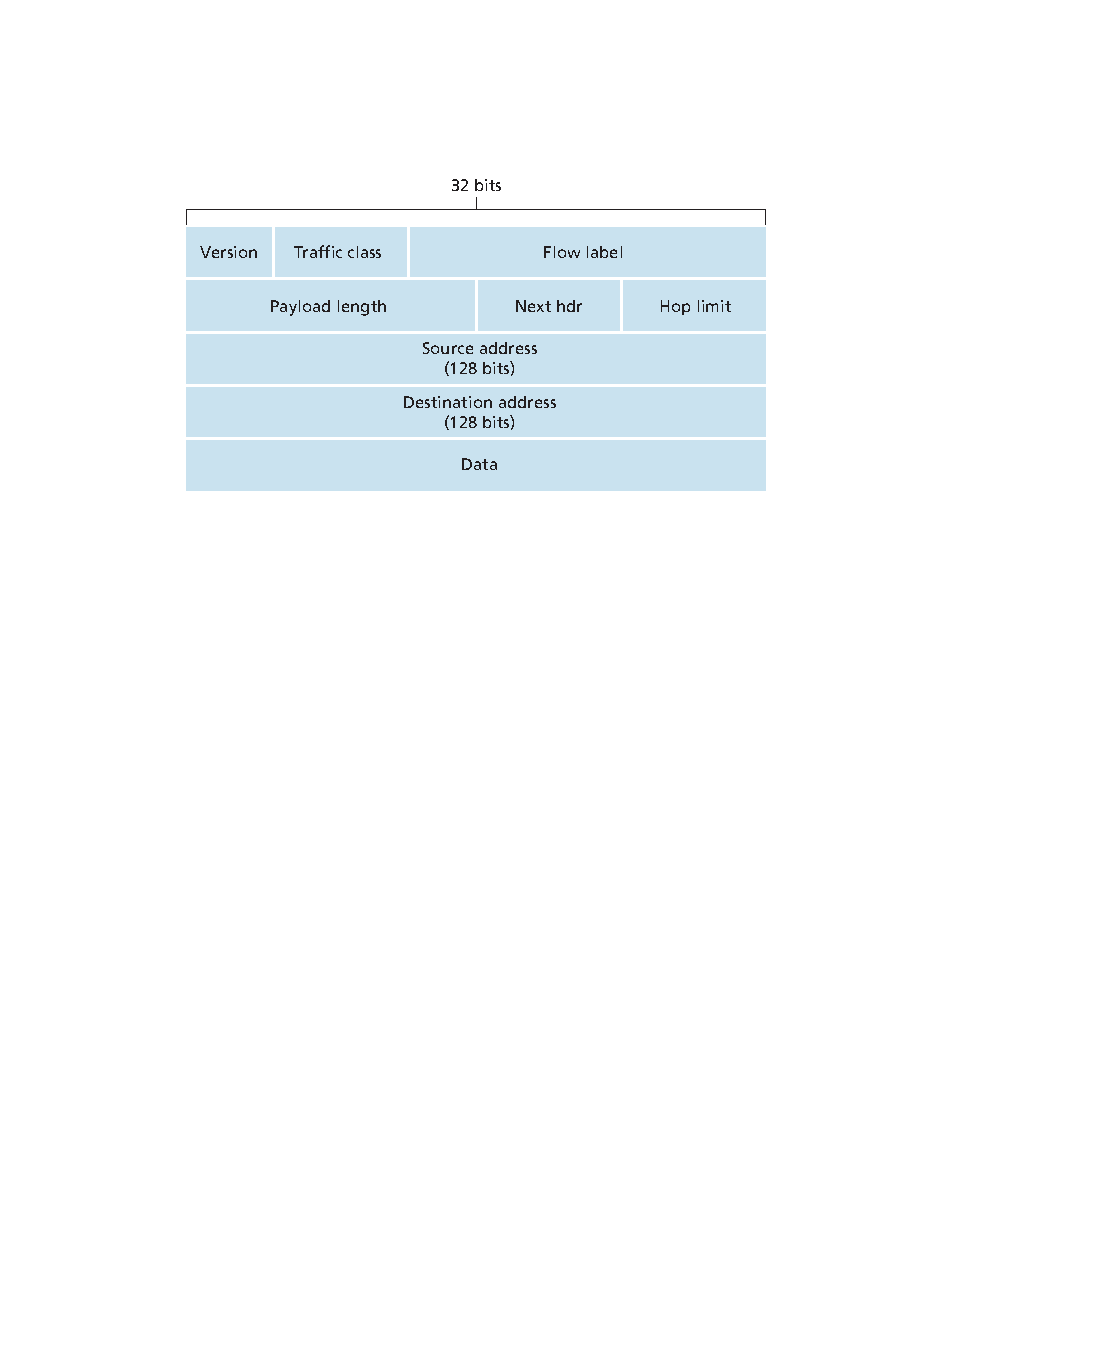
\includegraphics[width=0.6\textwidth]{kurose-04-24}
  \end{figure}
}
\end{frame}

\begin{frame}
  \frametitle{IP version 6 (IPv6)}
  \begin{exampleblock}{Principais avanços}
    \begin{enumerate}
    \item {\bf Espaço de endereçamento} - $2^{128}$ (de $2^{32}$ do IPv4).
    \item {\bf Melhor desempenho de roteamento} - sem soma de verificação e sem fragmentação.
    \item {\bf Suporte a tempo rea}l e outros serviços.
    \item {\bf Evolução futura} - campo \emph{próximo cabeçalho} (\emph{next hdr}).
    \item Difusão seletiva (\emph{multicast}) e {\bf não-seletiva} (\alert{anycast}).
    \item {\bf Segurança} - até agora, só suportado na camada de aplicação.
    \end{enumerate}
  \end{exampleblock}
\end{frame}

%-----------------------------------------------------------------------------%
\subsection{Camada de transporte}
%-----------------------------------------------------------------------------%

\begin{frame}
  \frametitle{Protocolos de transporte}
  \textbf{Última camada básica}: fornece todas as funcionalidades que os níveis abaixo não fornecem para um uso razoável 
  por uma aplicação de rede.
  \begin{block}{Protocolos de Internet \emph{de facto}}
    \begin{itemize}
    \item \blue{TCP} ({\bf Transmission Control Protocol}) -  orientado a conexão, confiável, controle de fluxo, sequencial.
    % TODO: UDP ordenado ?
    \item \blue{UDP} ({\bf Universal Datagram Protocol}) - sem conexão, não confiável, não ordernado.
    \end{itemize}
  \end{block}
  \pause
  \begin{alertblock}{Nota}
    Ambos são cliente-servidor.
%    IP multicasting é considerado um serviço disponível por padrão (o que pode ser perigoso).
  \end{alertblock}
\end{frame}

\begin{frame}
  \frametitle{Níveis de dados}
  \begin{enumerate}
  \item {\bf Nível 1 (física)} - bit stream.
  \item {\bf Nível 2 (enlace)} - frames.
  \item {\bf Nível 3 (rede)} - packets.
  \item {\bf Nível 4 (transporte)} - TPDU (\emph{Transport Protocol Data Unit})
    \begin{itemize}
    \item Segmentos (TCP).
    \item Datagramas (UDP).
    \end{itemize}
  \end{enumerate}
  %
%  \pause
%  %
%  \begin{block}{Portas e Sockets}
%    {\bf Port} - um número de 1 -- 65535.\\
%    {\bf Socket}
%    \begin{itemize}
%    \item Identifica um ponto final (\emph{endpoint}) em uma comunicação.
%    \item Caracterizado pela combinação:
%      \begin{itemize}
%      \item Tipo de protocolo (TCP, UDP, ....).
%      \item Endereço IP local.
%      \item Porta local.
%      \end{itemize}
%    \end{itemize}
%  \end{block}
\end{frame}

\begin{frame}
  \frametitle{Portas e Sockets}
  {\bf Port} - um número de 1 -- 65535, regidos pela IANA.
  \begin{itemize}
  \item Portas bem conhecidas ficam entre 0 -- 1024.
  \item Portas registradas ficam entre 1024 -- 49151.
  \item Portas dinâmicas/privadas entre 49152 -- 65535.
  \end{itemize}
  %
  {\bf Socket}
  \begin{itemize}
  \item Identifica um ponto final (\emph{endpoint}) em uma comunicação.
  \item Caracterizado pela combinação:
    \begin{itemize}
    \item Tipo de protocolo (TCP, UDP, ....).
    \item Endereço IP local.
    \item Porta local.
    \end{itemize}
  \end{itemize}
\end{frame}
%---------------------------------------------------------------------
\begin{frame}[fragile]
  \frametitle{Constantes}
\begin{lstlisting}
socket.socket(family=AF_INET,type=SOCK_STREAM, proto=0, fileno=None)
\end{lstlisting}
\begin{itemize}
\item \textbf{Family}:
  \begin{itemize}
    \item \texttt{AF\_UNIX}, \texttt{AF\_LOCAL} - comunicação local
    \item \texttt{AF\_INET} - protocolos de internet IPv4
    \item \texttt{AF\_INET6} - protocolos de internet IPv6
  \end{itemize}
\item \textbf{Type}:
  \begin{itemize}
    \item \texttt{SOCK\_STREAM} - TCP (orientando a conexão)
    \item \texttt{SOCK\_DGRAM} - UDP
  \end{itemize}
\end{itemize}
\end{frame}
%---------------------------------------------------------------------
\begin{frame}
  \frametitle{Protocolo UDP}
  \begin{itemize}
  \item Mais rápido em termos de desempenho porque não mantem conexões.
  \item Adiciona muito pouco ao IP.
  \item {\bf Não é confiável} - não garante envio de mensagens nem sua ordem.
  \item Uso - NFS, DNS, DHCP, jogos, streamming de audio e video.
  \end{itemize}
  %
  \begin{exampleblock}{Vantagens}
    \begin{enumerate}
    \item {\bf Controle fino} de dados enviados e recebidos.
    \item {\bf Sem conexões} (\textit{connectionless}) - sem custo para estabelecer conexões.
    \item {\bf Sem estado de conexão}.
    \item {\bf Header pequeno} - TCP adiciona 20 bytes, enquanto o UDP adiciona 8 bytes.
    \end{enumerate}
  \end{exampleblock}
\end{frame}

\begin{frame}
  \frametitle{Protocolo UDP}
\alt<presentation>
{
  \begin{center}
  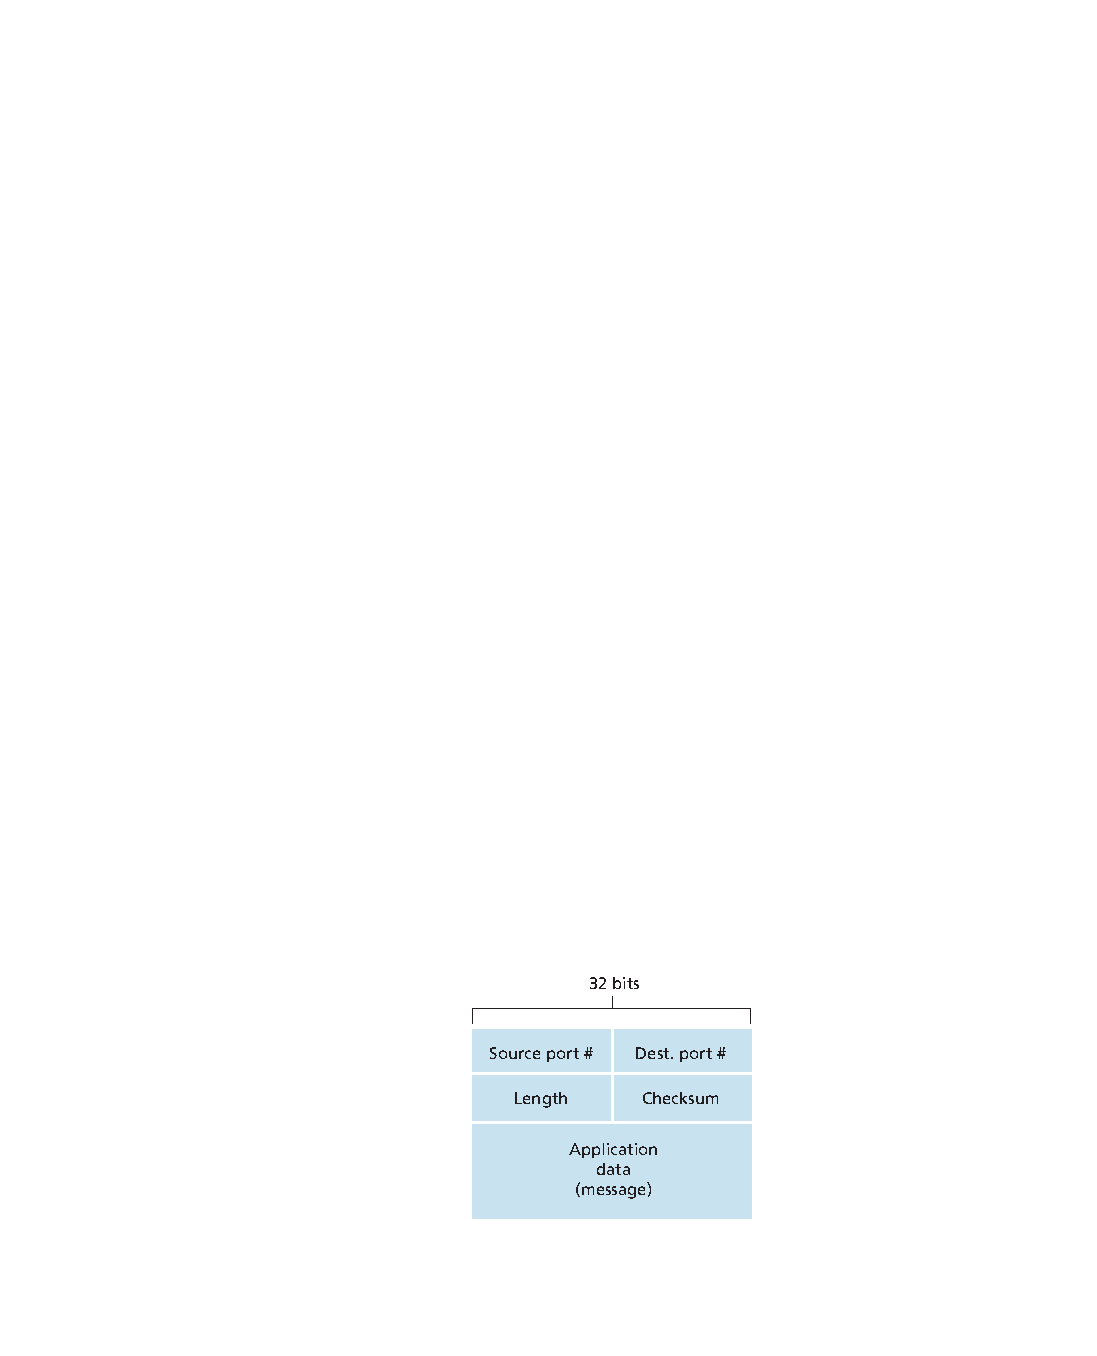
\includegraphics[scale=1.5]{kurose-03-07}
  \end{center}
}
{
  \begin{center}
  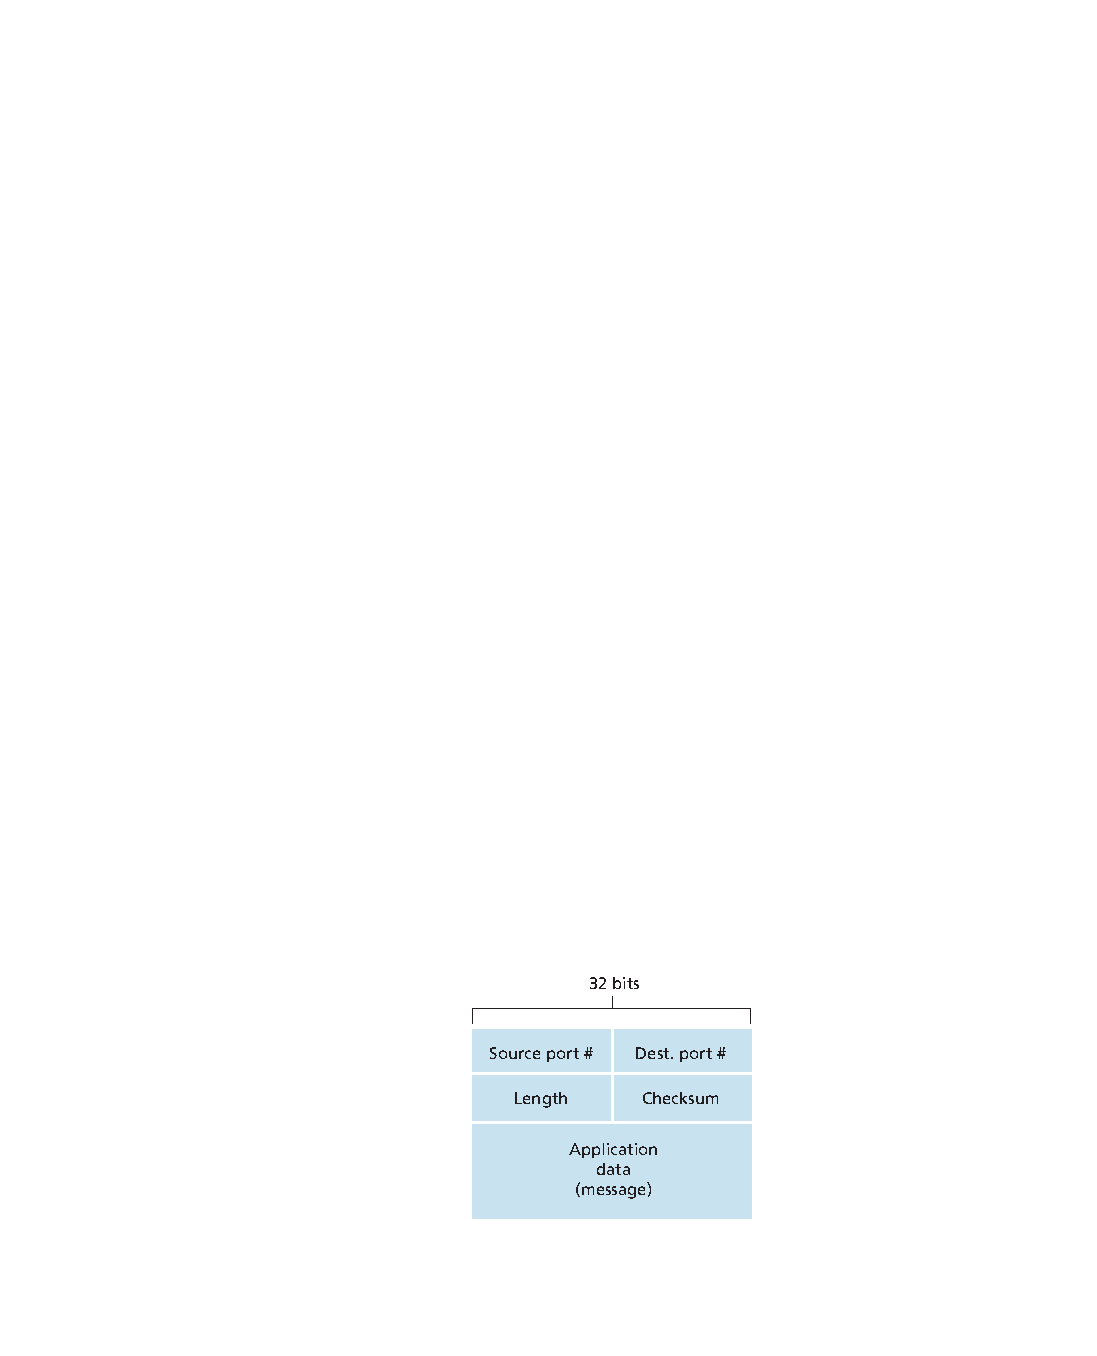
\includegraphics[scale=1]{kurose-03-07}
  \end{center}
}
\end{frame}

\begin{frame}[fragile]
  \frametitle{UDP em Python}
  {\bf Parte do envio:}
\begin{lstlisting}
#!/usr/bin/env python3
import socket

udp_ip = '127.0.0.1'
udp_port = 5005
message = 'Hello hello'

print("UDP target IP:" + udp_ip)
print("UDP target port: " + str(udp_port))
print("Messagem: " + message)

sock = socket.socket(socket.AF_INET, socket.SOCK_DGRAM)
sock.sendto(str.encode(message), (udp_ip, udp_port))
\end{lstlisting}
\end{frame}

\begin{frame}[fragile]
  \frametitle{UDP em Python}
  {\bf Parte do recebimento:}
\begin{lstlisting}
#!/usr/bin/env python3
import socket

udp_ip = '127.0.0.1'
udp_port = 5005
message = 'Hello hello'

sock = socket.socket(socket.AF_INET, socket.SOCK_DGRAM)
sock.bind((udp_ip, udp_port))

while True:
  data, addr = sock.recvfrom(1024) 
  print("Received: " + str(data))
\end{lstlisting}
\end{frame}

\begin{frame}
  \frametitle{Protocolo TCP}
  \begin{itemize}
  \item Protocolo baseado na comunicação permanente entre um cliente e um servidor.
  \end{itemize}
  %
  \begin{exampleblock}{Características}
    \begin{enumerate}
    \item {\bf Full-duplex} - transmissão nos dois sentidos.
    \item {\bf Point-to-point} - único remetente e único destinatário.
    \item {\bf Three-way handshake} - estabelece conexão em três passos.
    \item {\bf Ordenado} - ordem é garantida.
    \item {\bf Controle de fluxo} - caso o receptor é mais lento.
    \item {\bf Não tem} - timer, vazão mínima garantida, segurança.
    \end{enumerate}
  \end{exampleblock}
\end{frame}
%---------------------------------------------------------------------
\begin{frame}
  \frametitle{Protocolo TCP}
  \begin{center}
  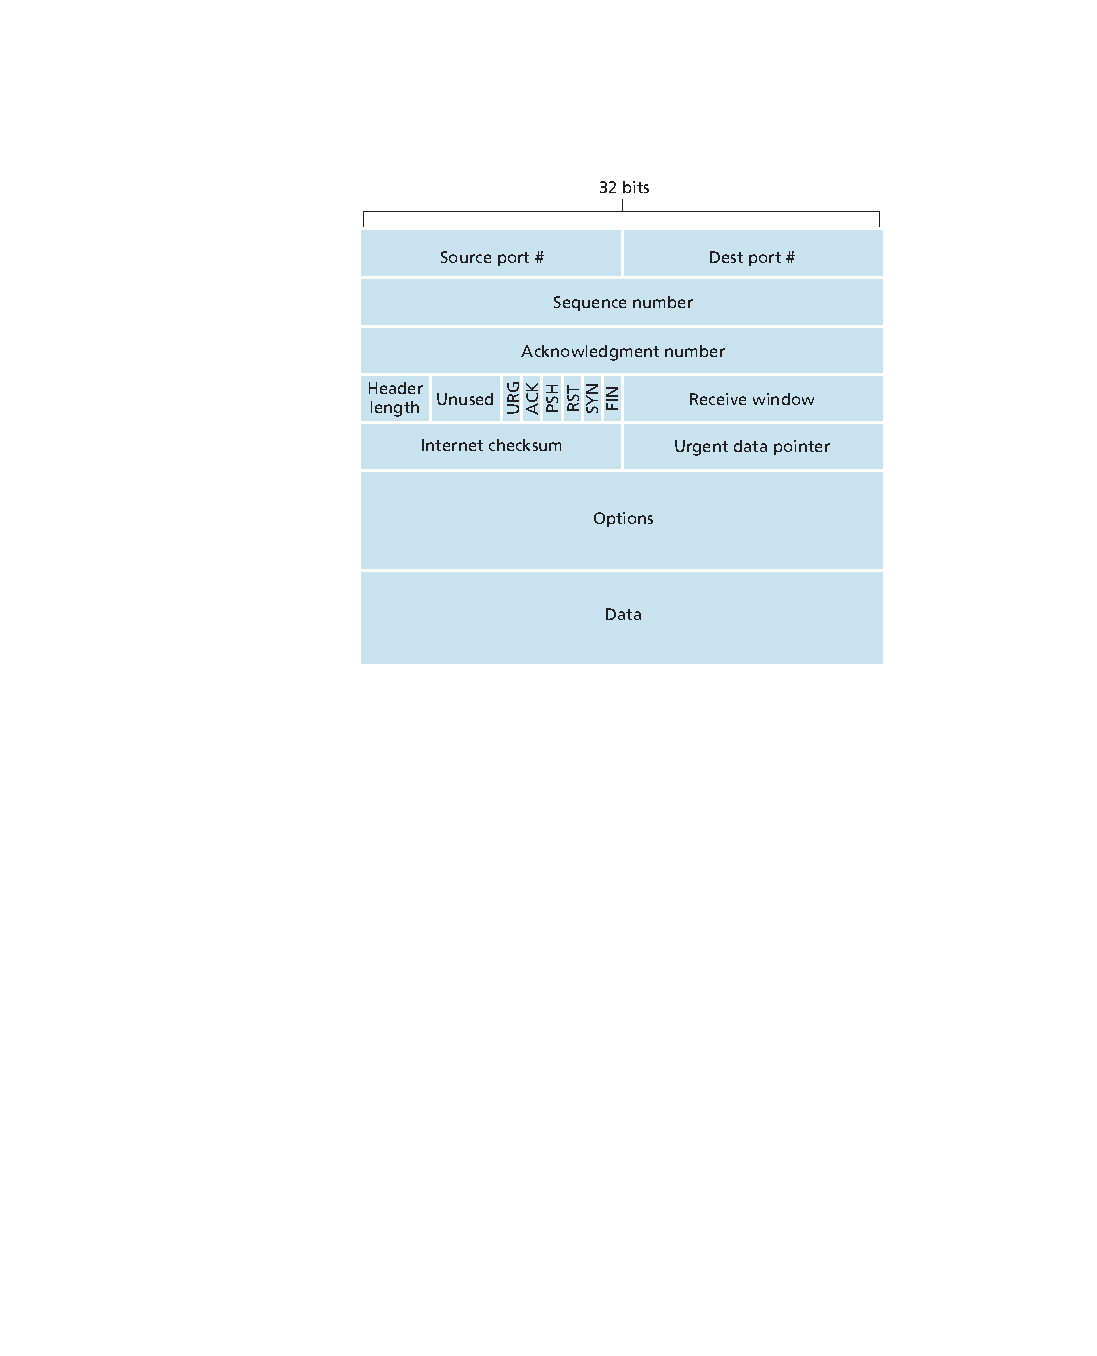
\includegraphics[scale=0.8]{kurose-03-29}
  \end{center}
\end{frame}
%---------------------------------------------------------------------
\begin{frame}[fragile]
  \frametitle{Servidor TCP}
\begin{lstlisting}
#!/usr/bin/env python3
import socket

host = 'localhost'
port = 50007
s = socket.socket(socket.AF_INET, socket.SOCK_STREAM)
s.bind((host, port))
s.listen(1)
conn, addr = s.accept()
with conn:
    print('Connected by', addr)
    while True:
        data = conn.recv(1024)
        if not data:
            break
        conn.sendall(data)
\end{lstlisting}
\end{frame}

\begin{frame}[fragile]
  \frametitle{Cliente TCP}
\begin{lstlisting}
#!/usr/bin/env python3
import socket

host = 'localhost'
port = 50007

s = socket.socket(socket.AF_INET, socket.SOCK_STREAM)
s.connect((host, port))
s.sendall(b'Hello, world')
data = s.recv(1024)
print('Received', repr(data))
\end{lstlisting}
\end{frame}

%-----------------------------------------------------------------------------%
\subsection{Camada de aplicação}
%-----------------------------------------------------------------------------%

\begin{frame}
  \frametitle{Protocolos de níveis mais altos}
  \begin{itemize}
  \item Na prática, acima da camada de transporte, somente a camada de aplicação é usada.
  \item Tudo acima dessa camada foi agrupado.
  \end{itemize}
  %
  \begin{block}{Protocolos de mais alto nível}
    \begin{itemize}
    \item \textbf{Sessão} -  Versão aprimorada da camada de transporte, que faz
      controle de diálogo e sincronização, raro suporte.
    \item \textbf{Apresentação} - Significado dos bits, define formato da mensagem.
    \item \textbf{Aplicação} - Pela  OSI era para conter um conjunto de aplicações padronizadas
      de rede como email, transferência de arquivos e terminal. Mas ela se tornou repositório
      para todas as aplicações e protocolos restantes.
    \end{itemize}
  \end{block}
\end{frame}

\begin{frame}
  \frametitle{Protocolos de níveis mais altos}
  \begin{itemize}
  \item O que falta nessa camada é uma clara distinção entre \textbf{aplicações}, \textbf{protocolos 
    específicos de aplicação} e \textbf{protocolos de uso geral}.
  \end{itemize}
  \begin{exampleblock}{Exemplos}
    \begin{itemize}
    \item \textbf{File Transfer Protocol (FTP)} - transferência de arquivos entre cliente e servidor. Não confundir
      com a aplicação \texttt{ftp}.
    \item \textbf{HyperText Transfer Protocol (HTTP)} - transferência de páginas Web. Implementado em 
      browsers Web (cliente) e servidores Web (servidor). Porém não é somente vínculado a Web como em objetos
      remotos em Java.
    \end{itemize}
  \end{exampleblock}
\end{frame}

\begin{frame}
  \frametitle{Protocolos de middleware}
  \begin{block}{Observação}
  Middleware é concebido para prover \textbf{protocolos de uso geral} que podem ser usados por 
  diferentes aplicações.
  \end{block}
  \begin{exampleblock}{Um rico conjunto de \textbf{protocolos de comunicação}}
    \begin{itemize}
    \item \textbf{(Un)marshaling} de dados, para sistemas integrados.
    \item \textbf{Protocolos de nomeação} para compartilhamente fácil de recursos.
    \item \textbf{Protocolos de segurança} para comunicação segura.
    \item \textbf{Mecanismo de escalabilidade} como repliação e caching.
    \end{itemize}
  \end{exampleblock}
\end{frame}

\begin{frame}
  \frametitle{Protocolos de middleware}
  \begin{block}{Observação}
  Middleware é concebido para prover \textbf{protocolos de uso geral} que podem ser usados por 
  diferentes aplicações.
  \end{block}
  %
  \begin{exampleblock}{Serviços de comunicação de alto nível}
    \begin{itemize}
    \item Chamada de procedimentos remotos.
    \item Invocar objetos remotos.
    \item Estabelecer e sincronizar fluxos para dados em tempo real.
    \item Oferecer serviços multicast confiáveis.
    \end{itemize}
  \end{exampleblock}
\end{frame}

%-----------------------------------------------------------------------------%
\subsection{Domain Name Server (DNS)}
%-----------------------------------------------------------------------------%

\begin{frame}
  \frametitle{Domain Name Server (DNS)}
  \begin{itemize}
  \item Traduzir nomes (\emph{hostname}) para endereços IP.
  \item Serviço de diretório, ou banco de dados distribuído, em hierarquia.
  \item Executa sobre o protocolo TCP ou UDP porta 53.
  \end{itemize}
  %
  \pause 
  %
  \begin{exampleblock}{Outros serviços}
    \begin{itemize}
    \item {\bf Host aliasing} - ``apelidos'' de um host (o original é o \textbf{canonical hostname}).
    \item {\bf Mail server aliasing} - servidor Web e Mail podem ter o mesmo nome.
    \item {\bf Load distribution} - distribuição de trabalho, ou seja, quando um cliente consulta
    um nome com vários IPs, ele retorna todos e alterna a ordem deles. O cliente normalmente usa o
    primeiro IP.
    \end{itemize}
  \end{exampleblock}
\end{frame}

\begin{frame}
  \frametitle{Registros DNS}
  \begin{itemize}
	  \item \textbf{SOA} -  \emph{Start of Authority}, informações de domínio como serial number, e prazos.
	  \item \textbf{NS} - \emph{name server}.
	  \item \textbf{A ou AAAA} - \emph{IP address} IPv4 ou IPv6.
	  \item \textbf{MX} - \emph{SMTP mail exchangers}, servidor de email do domínio.
	  \item \textbf{PTR} - \emph{reverse DNS lookup}.
	  \item \textbf{CNAME} - \emph{domain name aliases}.
  \end{itemize}
\end{frame}

\begin{frame}
  \frametitle{Hierarquia DNS}
  \begin{center}
  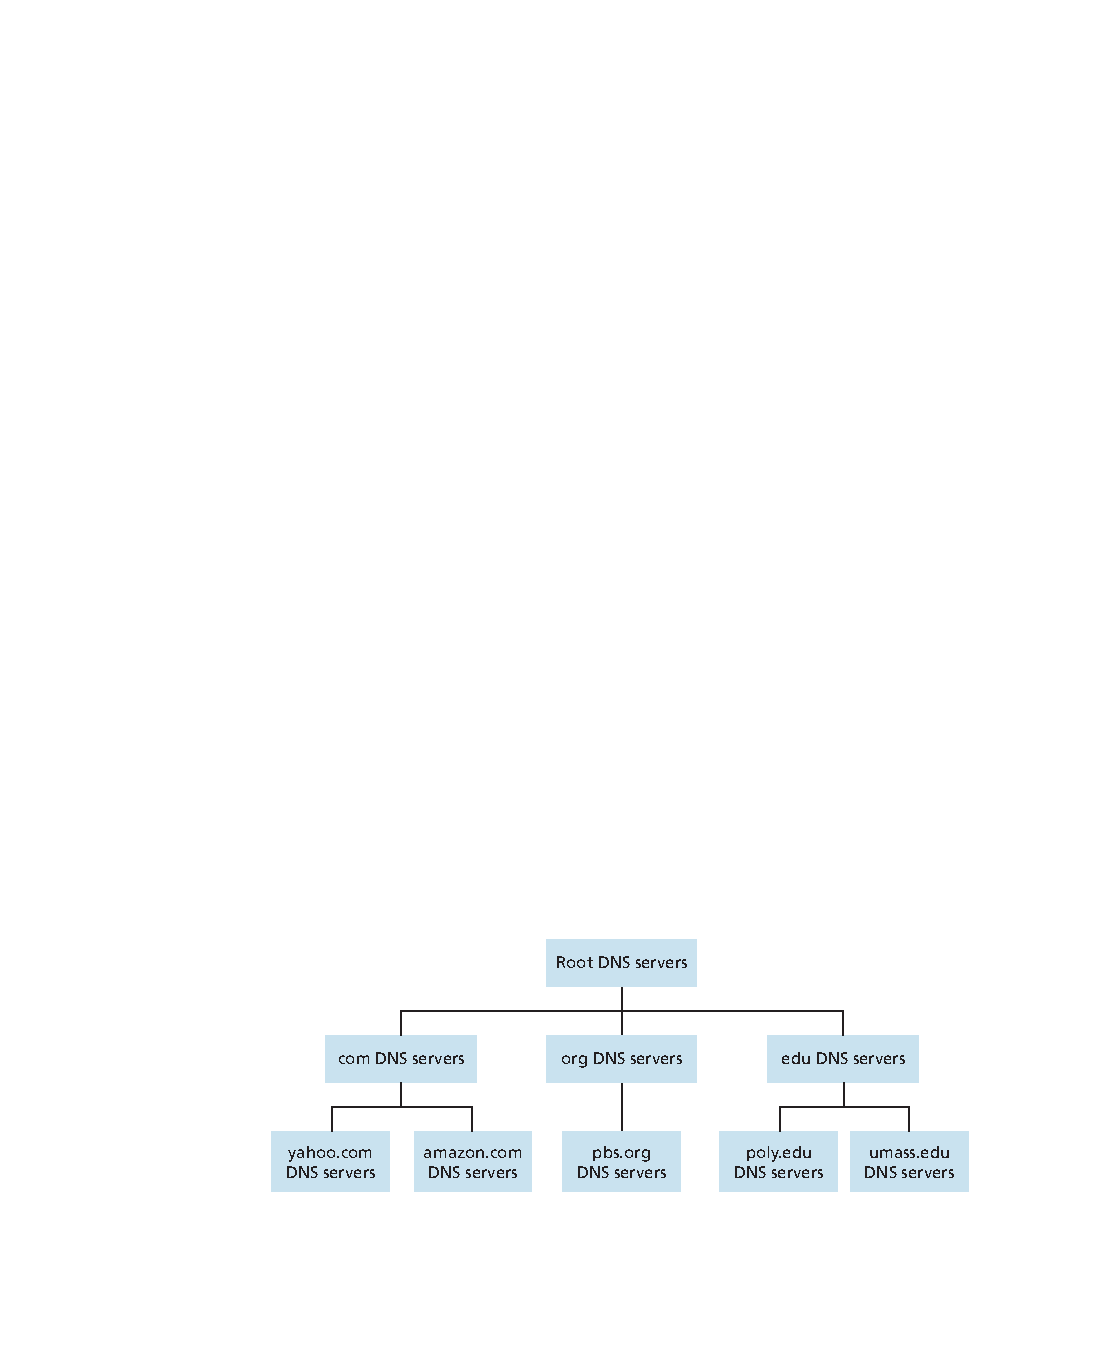
\includegraphics[scale=0.9]{kurose-02-19}
  \end{center}
\end{frame}

\begin{frame}[fragile]
  \frametitle{Hierarquia DNS}
  \begin{itemize}
  \item {\bf Root DNS servers} - 13 servidores raízes, maioria na América do Norte. Porém cada servidor
    é uma rede de duplicatas sendo todos aproximadamente 247 servidores.
  \item {\bf Top-level domain (TLD) servers} - Domínios \verb+com+, \verb+org+, \verb+net+,
    \verb+edu+ e \verb+gov+, e de países como \verb+uk+, \verb+fr+, \verb+ca+, \verb+br+, etc.
  \item {\bf Authoritative DNS servers} - Organizações com acesso aberto devem prover entradas
    DNS. Universidades e grandes companias mantem seus próprios servidores DNS.
  \end{itemize}
\end{frame}

\begin{frame}
  \frametitle{Servidores raiz do DNS}
  \begin{center}
  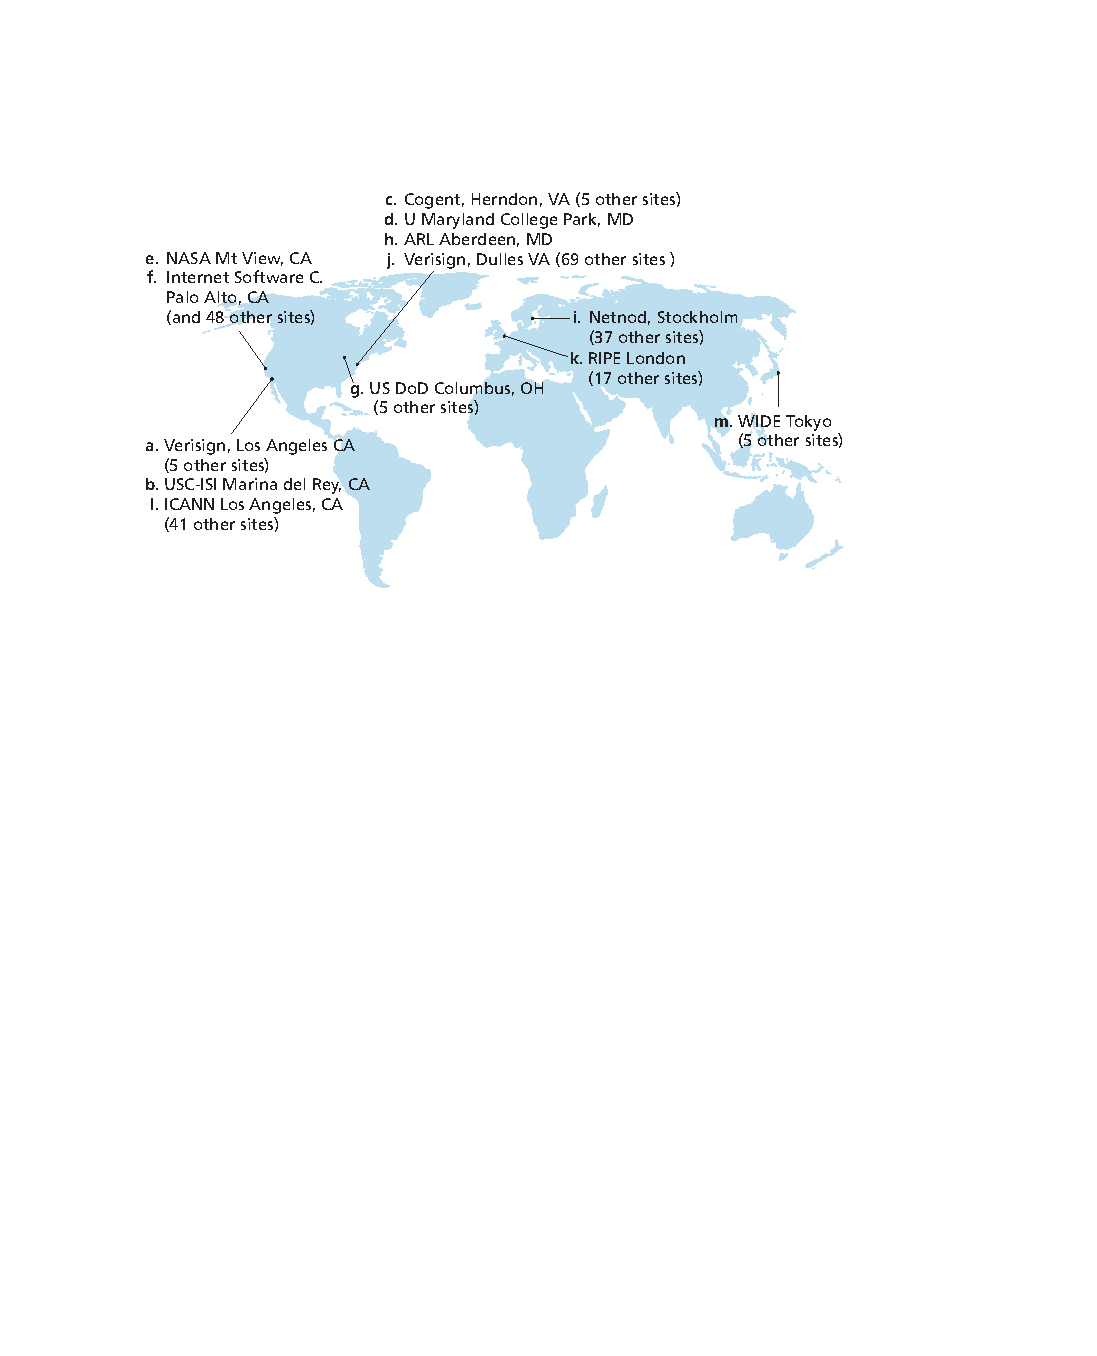
\includegraphics[scale=0.9]{kurose-02-20}
  \end{center}
\end{frame}

%%%%%%%%%%%%%%%%%%%%%%%%%%%%%%%%%%%%%%%%%%%%%%%%%%%%%%%%%%%%%%%%%%%%%%%%%%%%%%%
\section{Ferramentas}
%%%%%%%%%%%%%%%%%%%%%%%%%%%%%%%%%%%%%%%%%%%%%%%%%%%%%%%%%%%%%%%%%%%%%%%%%%%%%%%

%-----------------------------------------------------------------------------%
\subsection{Ping}
%-----------------------------------------------------------------------------%

\begin{frame}[fragile]
  \frametitle{Ping}
\begin{itemize}
	\item Envia pacotes ICMP (\emph{Internet Control Message Protocol}).
	\item \textbf{TTL} - \emph{Time to live} ou \emph{hop limit}
	\item Round-trip time
\end{itemize}
\begin{verbatim}
ping -c 5 8.8.8.8
PING 8.8.8.8 (8.8.8.8) 56(84) bytes of data.
64 bytes from 8.8.8.8: icmp_seq=1 ttl=52 time=28.7 ms
64 bytes from 8.8.8.8: icmp_seq=2 ttl=52 time=26.5 ms
64 bytes from 8.8.8.8: icmp_seq=3 ttl=52 time=26.7 ms
64 bytes from 8.8.8.8: icmp_seq=4 ttl=52 time=26.5 ms
64 bytes from 8.8.8.8: icmp_seq=5 ttl=52 time=26.7 ms

--- 8.8.8.8 ping statistics ---
5 packets transmitted, 5 received, 0% packet loss, time 11ms
rtt min/avg/max/mdev = 26.467/27.015/28.702/0.868 ms
\end{verbatim}
\end{frame}
%---------------------------------------------------------------------
\subsection{Dig}
%-----------------------------------------------------------------------------%
\begin{frame}[fragile]
	\frametitle{Domain Information Groper (dig)}
\begin{itemize}
	\item Consultas ao registro DNS.
\end{itemize}
\begin{small}
\begin{verbatim}
$ dig www.inf.ufsm.br
; <<>> DiG 9.11.4-3ubuntu5.3-Ubuntu <<>> www.inf.ufsm.br
;; global options: +cmd
;; Got answer:
;; ->>HEADER<<- opcode: QUERY, status: NOERROR, id: 38319
;; flags: qr rd ra; QUERY: 1, ANSWER: 1, AUTHORITY: 0, ADDITIONAL: 1

;; OPT PSEUDOSECTION:
; EDNS: version: 0, flags:; udp: 65494
;; QUESTION SECTION:
;www.inf.ufsm.br.		IN	A

;; ANSWER SECTION:
www.inf.ufsm.br.	7193	IN	A	200.18.42.2

;; Query time: 0 msec
;; SERVER: 127.0.0.53#53(127.0.0.53)
;; WHEN: seg mai 06 14:38:50 -03 2019
;; MSG SIZE  rcvd: 60
\end{verbatim}
\end{small}
\end{frame}
%-----------------------------------------------------------------------------%
\begin{frame}[fragile]
	\frametitle{Domain Information Groper (dig)}
\begin{small}
\begin{verbatim}
$ dig inf.ufsm.br ns
; <<>> DiG 9.11.4-3ubuntu5.3-Ubuntu <<>> inf.ufsm.br ns
;; global options: +cmd
;; Got answer:
;; ->>HEADER<<- opcode: QUERY, status: NOERROR, id: 8007
;; flags: qr rd ra; QUERY: 1, ANSWER: 1, AUTHORITY: 0, ADDITIONAL: 1

;; OPT PSEUDOSECTION:
; EDNS: version: 0, flags:; udp: 65494
;; QUESTION SECTION:
;inf.ufsm.br.			IN	NS

;; ANSWER SECTION:
inf.ufsm.br.		6241	IN	NS	dns.inf.ufsm.br.

;; Query time: 0 msec
;; SERVER: 127.0.0.53#53(127.0.0.53)
;; WHEN: seg mai 06 14:42:01 -03 2019
;; MSG SIZE  rcvd: 58
\end{verbatim}
\end{small}
\end{frame}
%-----------------------------------------------------------------------------%
\begin{frame}[fragile]
	\frametitle{Domain Information Groper (dig)}
\begin{small}
\begin{verbatim}
 dig inf.ufsm.br mx

;; ANSWER SECTION:
inf.ufsm.br.		200	IN	MX	5 alt2.aspmx.l.google.com.
inf.ufsm.br.		200	IN	MX	1 aspmx.l.google.com.
inf.ufsm.br.		200	IN	MX	10 aspmx3.googlemail.com.
inf.ufsm.br.		200	IN	MX	5 alt1.aspmx.l.google.com.
inf.ufsm.br.		200	IN	MX	10 aspmx2.googlemail.com.
inf.ufsm.br.		200	IN	MX	10 aspmx5.googlemail.com.
inf.ufsm.br.		200	IN	MX	10 aspmx4.googlemail.com.

;; Query time: 1 msec
;; SERVER: 127.0.0.53#53(127.0.0.53)
;; WHEN: seg mai 06 15:05:12 -03 2019
;; MSG SIZE  rcvd: 219
\end{verbatim}
\end{small}
\end{frame}
%-----------------------------------------------------------------------------%
\subsection{Nmap}
%-----------------------------------------------------------------------------%
\begin{frame}[fragile]
	\frametitle{Network Mapper}
	\begin{itemize}
	\item Scanner de rede com diversas funcionalidades.
	\end{itemize}
\begin{small}
\begin{verbatim}
$ map 8.8.8.8
Starting Nmap 7.60 ( https://nmap.org ) at 2019-05-06 15:08 -03
Nmap scan report for google-public-dns-a.google.com (8.8.8.8)
Host is up (0.039s latency).
Not shown: 998 filtered ports
PORT    STATE SERVICE
53/tcp  open  domain
443/tcp open  https

Nmap done: 1 IP address (1 host up) scanned in 4.82 seconds
\end{verbatim}
\end{small}
\end{frame}
%-----------------------------------------------------------------------------%
\begin{frame}[fragile]
	\frametitle{Network Mapper}
	\begin{itemize}
	\item Scanner de rede com diversas funcionalidades.
	\end{itemize}
\begin{small}
\begin{verbatim}
$ nmap -p 22 8.8.8.8

Starting Nmap 7.60 ( https://nmap.org ) at 2019-05-06 15:37 -03
Nmap scan report for google-public-dns-a.google.com (8.8.8.8)
Host is up (0.034s latency).

PORT   STATE    SERVICE
22/tcp filtered ssh

Nmap done: 1 IP address (1 host up) scanned in 0.42 seconds
\end{verbatim}
\end{small}
\end{frame}
%-----------------------------------------------------------------------------%
\subsection{Sipcalc}
%-----------------------------------------------------------------------------%
\begin{frame}[fragile]
	\frametitle{IP Subnet Calculator}
\begin{small}
\begin{verbatim}
$ sipcalc  10.1.1.20/24
-[ipv4 : 10.1.1.20/24] - 0

[CIDR]
Host address		- 10.1.1.20
Host address (decimal)	- 167837972
Host address (hex)	- A010114
Network address		- 10.1.1.0
Network mask		- 255.255.255.0
Network mask (bits)	- 24
Network mask (hex)	- FFFFFF00
Broadcast address	- 10.1.1.255
Cisco wildcard		- 0.0.0.255
Addresses in network	- 256
Network range		- 10.1.1.0 - 10.1.1.255
Usable range		- 10.1.1.1 - 10.1.1.254
\end{verbatim}
\end{small}
\end{frame}
%-----------------------------------------------------------------------------%
\begin{frame}[fragile]
	\frametitle{IP Subnet Calculator}
\begin{small}
\begin{verbatim}
$ sipcalc  10.1.1.100/30
-[ipv4 : 10.1.1.100/30] - 0

[CIDR]
Host address		- 10.1.1.100
Host address (decimal)	- 167838052
Host address (hex)	- A010164
Network address		- 10.1.1.100
Network mask		- 255.255.255.252
Network mask (bits)	- 30
Network mask (hex)	- FFFFFFFC
Broadcast address	- 10.1.1.103
Cisco wildcard		- 0.0.0.3
Addresses in network	- 4
Network range		- 10.1.1.100 - 10.1.1.103
Usable range		- 10.1.1.101 - 10.1.1.102
\end{verbatim}
\end{small}
\end{frame}
%-----------------------------------------------------------------------------%
%%%%%%%%%%%%%%%%%%%%%%%%%%%%%%%%%%%%%%%%%%%%%%%%%%%%%%%%%%%%%%%%%%%%%%%%%%%%%%%
\section{Bibliografia}

\begin{frame}
  \frametitle{Bibliografia}
  \begin{itemize}
  \item {\bf Sistemas Distribuídos - Princípios e Paradigmas}, A. Tanenbaum e M. Steen, Cap. 4
  \item {\bf Sistemas Distribuídos - Conceitos e Projeto}, G. Coulouris, J. Dollimore, T. Kindberg e G. Blair, Cap. 3
  \item {\bf Computer Networking: A Top-Down Approach}, J. F. Kurose, K. W. Ross.
  \end{itemize}
\end{frame}

\end{document}
